\section{Selections}


\subsection{Event selections}

\begin{frame}{Event selection}
\smaller
    \begin{table}
        \centering
        \setlength{\tabcolsep}{1em}
        \renewcommand{\arraystretch}{1.5}
        \resizebox{0.95\textwidth}{!}{    \begin{tabular}{c|c|ccc|c|c}     
        \hline 
        trigger                & label  & $N_{\Pe}$ & $N_{\PGm}$ & $N_{\PGt}$   & \pt & other  \\
        \hline                                                                                      
        \multirow{4}{*}{\Pe}   & \cee   & 2         & 0          & 0            & $\pt^{\Pe(\Pe)}  > 30 \, (20)\GeV$ & OS, $|m_{\cee} - m_{\PZ}| > 15\GeV$   \\
                               & \cem   & 1         & 1          & 0            & $\pt^{\Pe(\PGm)} > 30 \, (10)\GeV$ & OS\\
                               & \cet   & 1         & 0          & 1            & $\pt^{\Pe(\PGth)}> 30 \, (20)\GeV$ & OS\\
                               & \ceh   & 1         & 0          & 0            & $\pt^{\Pe} > 30\GeV$               &    \\
        \hline                                                                      
        \multirow{4}{*}{\PGm}  & \cme   & 1         & 1          & 0            & $\pt^{\PGm(\Pe)}  > 25 \, (20)\GeV$ & OS \\
                               & \cmm   & 0         & 2          & 0            & $\pt^{\PGm(\PGm)} > 25 \, (10)\GeV$ & OS,$|m_{\cmm} - m_{\PZ}| > 15\GeV$  \\
                               & \cmt   & 0         & 1          & 1            & $\pt^{\PGm(\PGth)}> 25 \, (20)\GeV$ & OS \\
                               & \cmh   & 0         & 1          & 0            & $\pt^{\PGm} > 25\GeV$               &    \\\hline 
                        
    \end{tabular}}
    \end{table}
    % \small{ *) opposite sign (OS)}
    
    \begin{itemize}
        \item Channels are further split based on $n_j$ and $n_b$
        \item Baseline categories require
        \begin{itemize}
        \smaller
            \item $n_j\geq 2$ in $\ell\ell$ and $\ell \PGth$ channels,
            \item $n_j\geq 4$ in \ceh and \cmh channels,
        \end{itemize}
        with either $n_b=1$ or $n_b\geq2$, giving a high purity of \ttbar and \tW.
    \end{itemize}
    
    \footnotetext[1]{\tiny OS for opposite sign.}
    \footnotetext[2]{\tiny counting analysis uses $\pt^\PGm>30 \GeV$ for the leading muon in muon triggered channels to reduce QCD.}
\end{frame}




\begin{frame}{}
    Baseline categories with $n_b=1$
    \begin{block}{\smaller \PGm trigger}
    \begin{center}
        \centering
        \cme \qquad\qquad\qquad\quad \cmm \qquad\qquad\qquad\quad \cmt \qquad\qquad\qquad\quad \cmh \\
        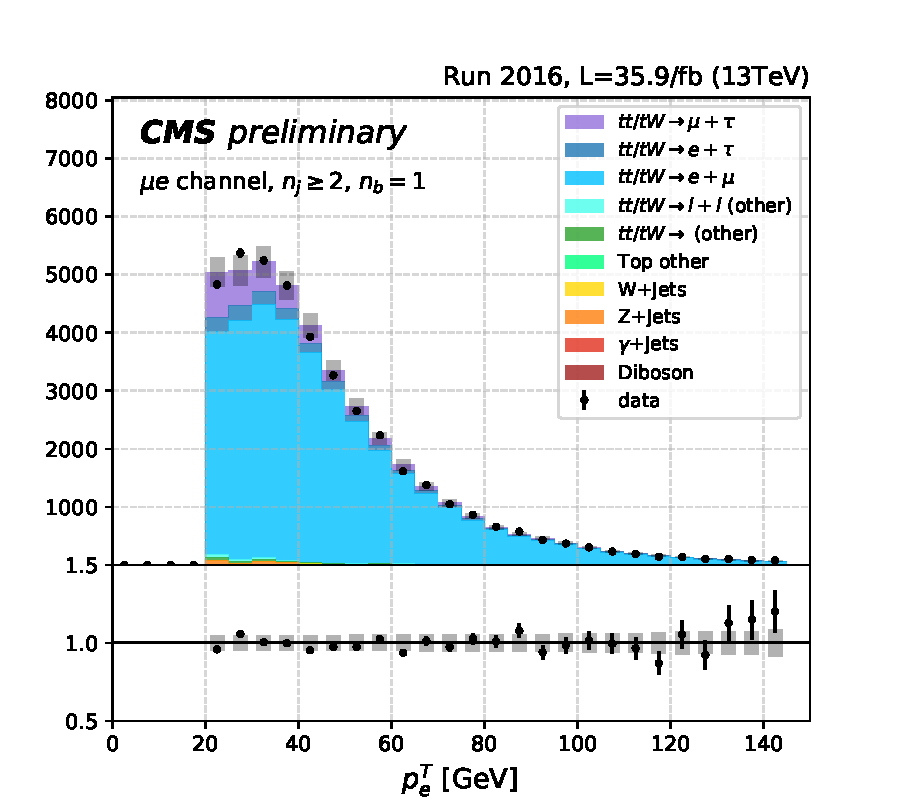
\includegraphics[width=0.24\textwidth]{chapters/Analysis/sectionPlots/figures/kinematics_pickles/emu/1b/emu_1b_lepton2_pt.pdf}
        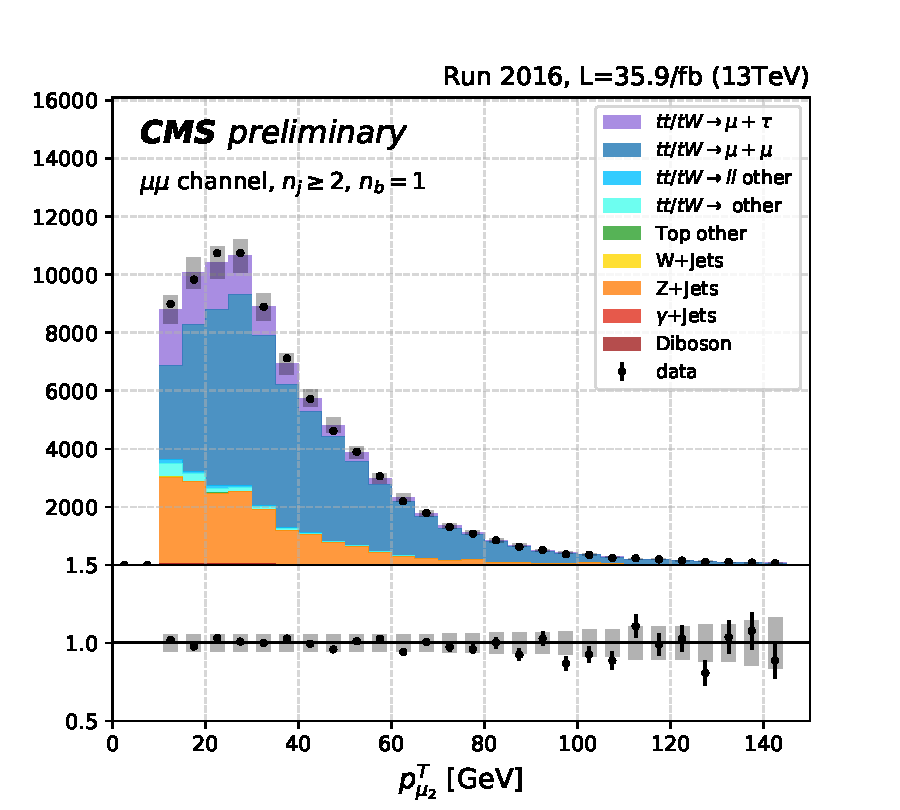
\includegraphics[width=0.24\textwidth]{chapters/Analysis/sectionPlots/figures/kinematics_pickles/mumu/1b/mumu_1b_lepton2_pt.pdf}
        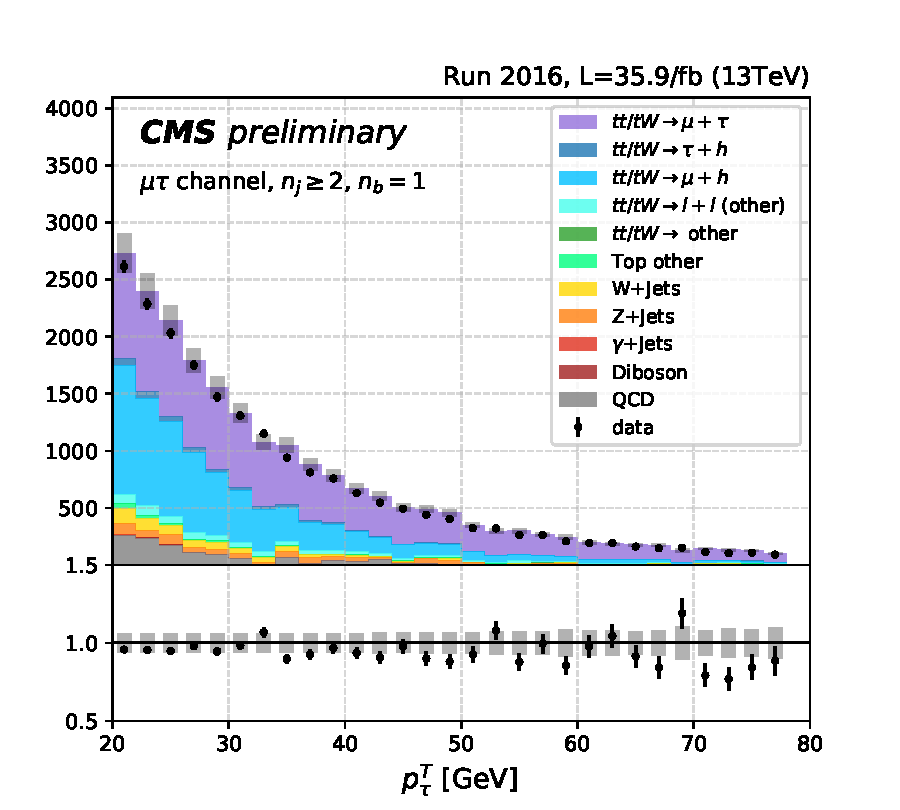
\includegraphics[width=0.24\textwidth]{chapters/Analysis/sectionPlots/figures/kinematics_pickles/mutau/1b/mutau_1b_lepton2_pt.pdf}
        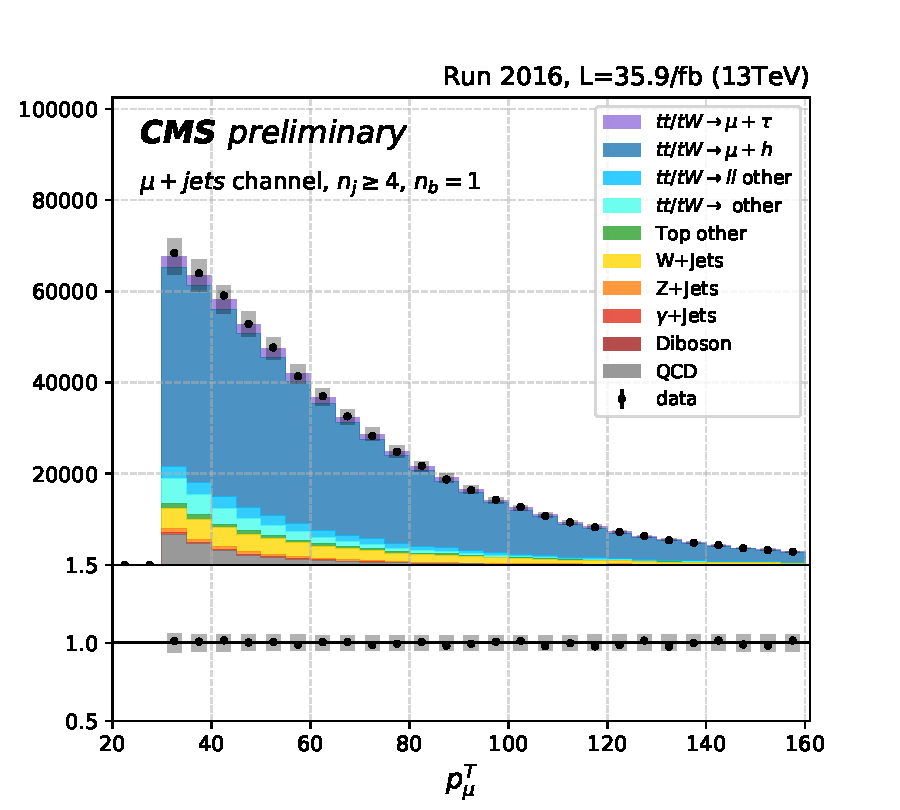
\includegraphics[width=0.24\textwidth]{chapters/Analysis/sectionPlots/figures/kinematics_pickles/mu4j/1b/mu4j_1b_lepton1_pt.pdf}
    \end{center}
    \end{block}
    
    \begin{block}{\smaller \Pe trigger}
    \begin{center}
        \cee \qquad\qquad\qquad\quad \cem \qquad\qquad\qquad\quad \cet \qquad\qquad\qquad\quad \ceh \\
        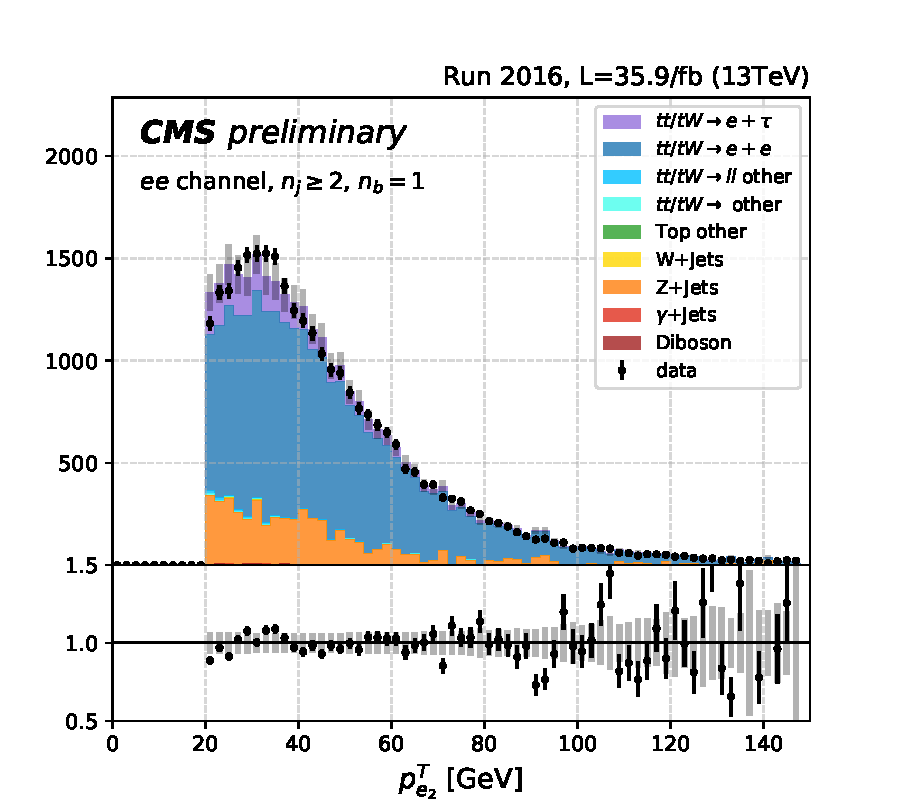
\includegraphics[width=0.24\textwidth]{chapters/Analysis/sectionPlots/figures/kinematics_pickles/ee/1b/ee_1b_lepton2_pt.pdf}
        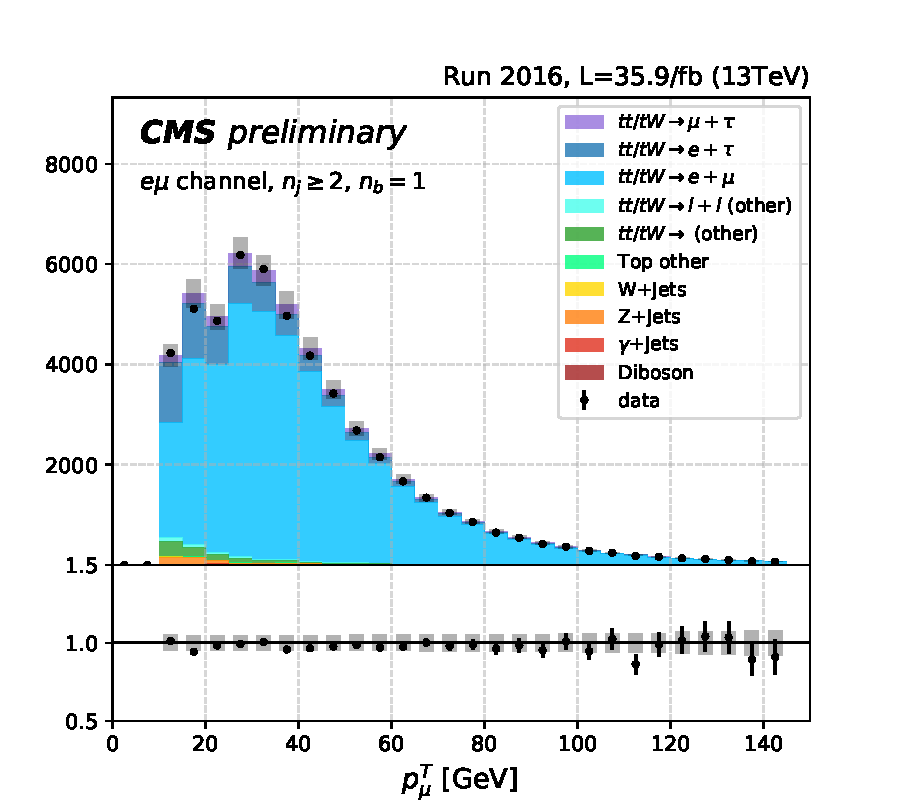
\includegraphics[width=0.24\textwidth]{chapters/Analysis/sectionPlots/figures/kinematics_pickles/emu2/1b/emu2_1b_lepton1_pt.pdf}
        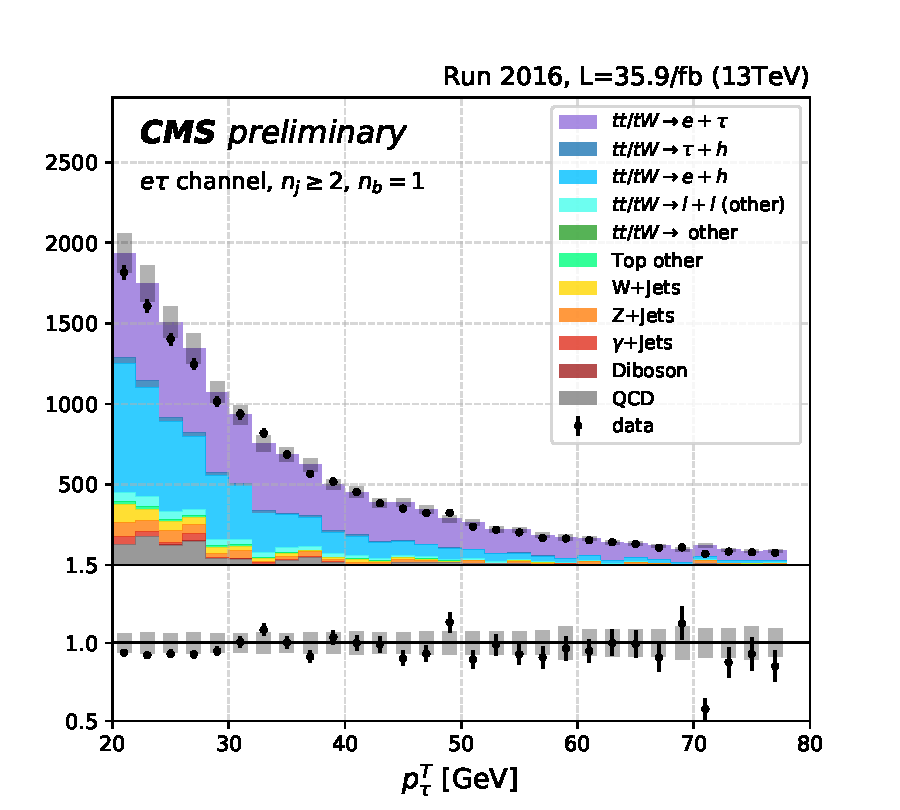
\includegraphics[width=0.24\textwidth]{chapters/Analysis/sectionPlots/figures/kinematics_pickles/etau/1b/etau_1b_lepton2_pt.pdf}
        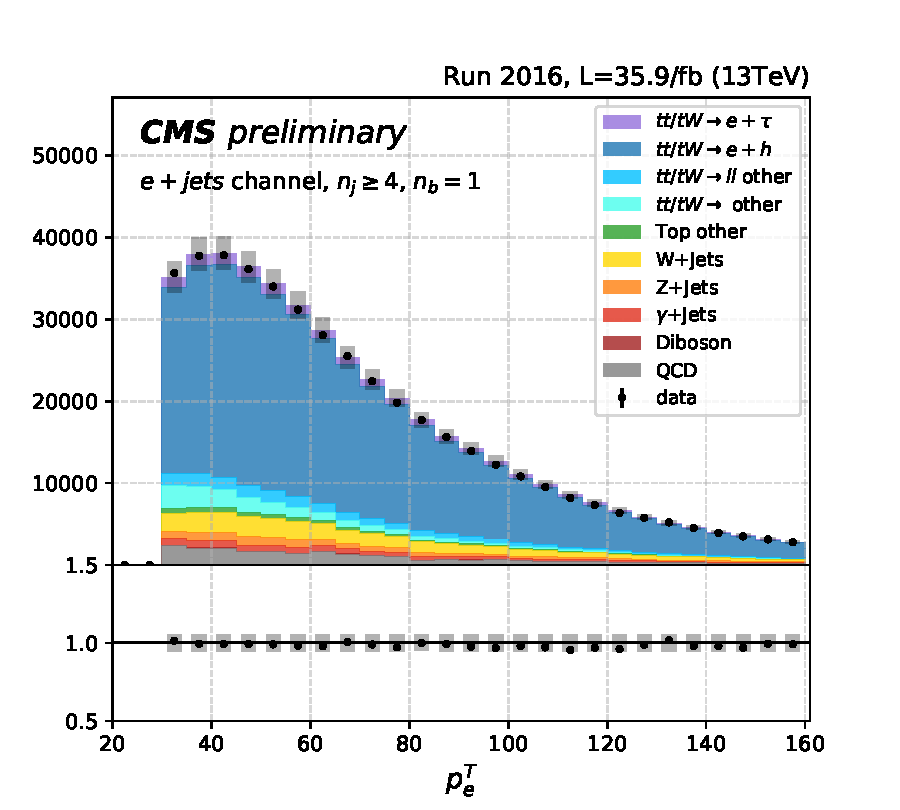
\includegraphics[width=0.24\textwidth]{chapters/Analysis/sectionPlots/figures/kinematics_pickles/e4j/1b/e4j_1b_lepton1_pt.pdf}
    \end{center}
    \end{block}
    
\end{frame}




\begin{frame}{}
    Baseline categories with $n_b\geq2$
    \begin{block}{\smaller \PGm trigger}
    \begin{center}
        \cme \qquad\qquad\qquad\quad \cmm \qquad\qquad\qquad\quad \cmt \qquad\qquad\qquad\quad \cmh \\
        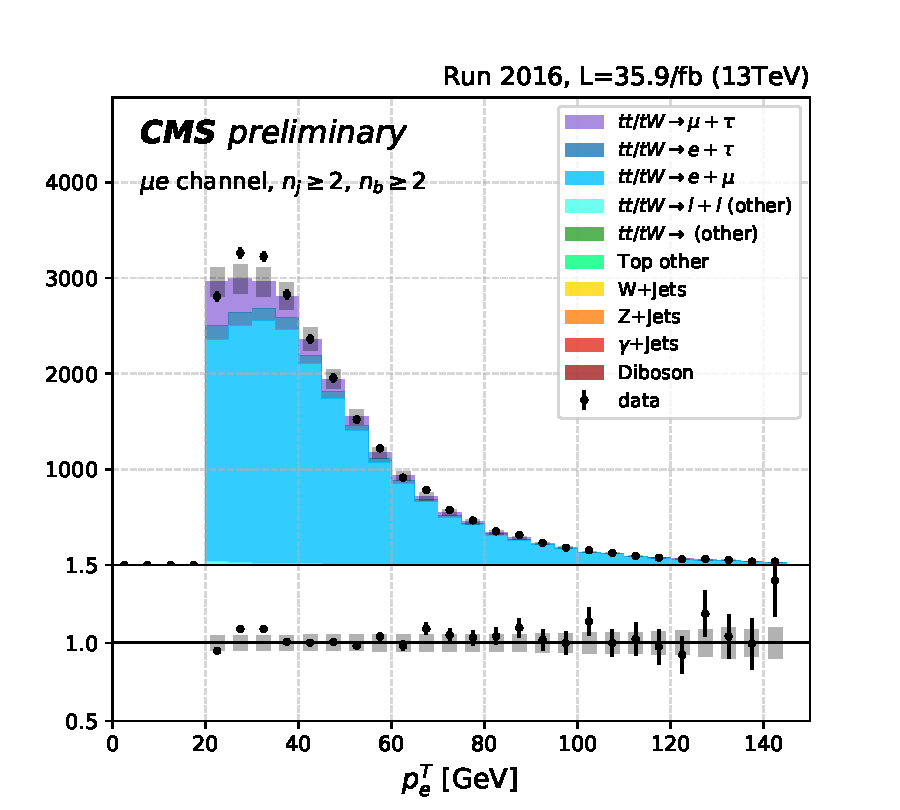
\includegraphics[width=0.24\textwidth]{chapters/Analysis/sectionPlots/figures/kinematics_pickles/emu/2b/emu_2b_lepton2_pt.pdf}
        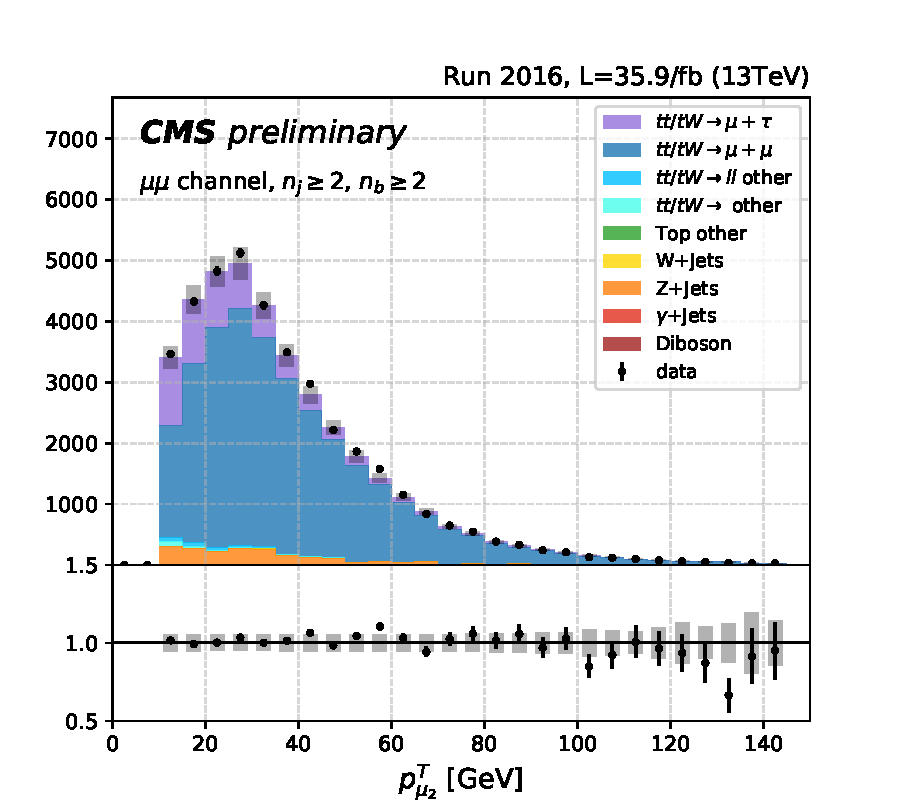
\includegraphics[width=0.24\textwidth]{chapters/Analysis/sectionPlots/figures/kinematics_pickles/mumu/2b/mumu_2b_lepton2_pt.pdf}
        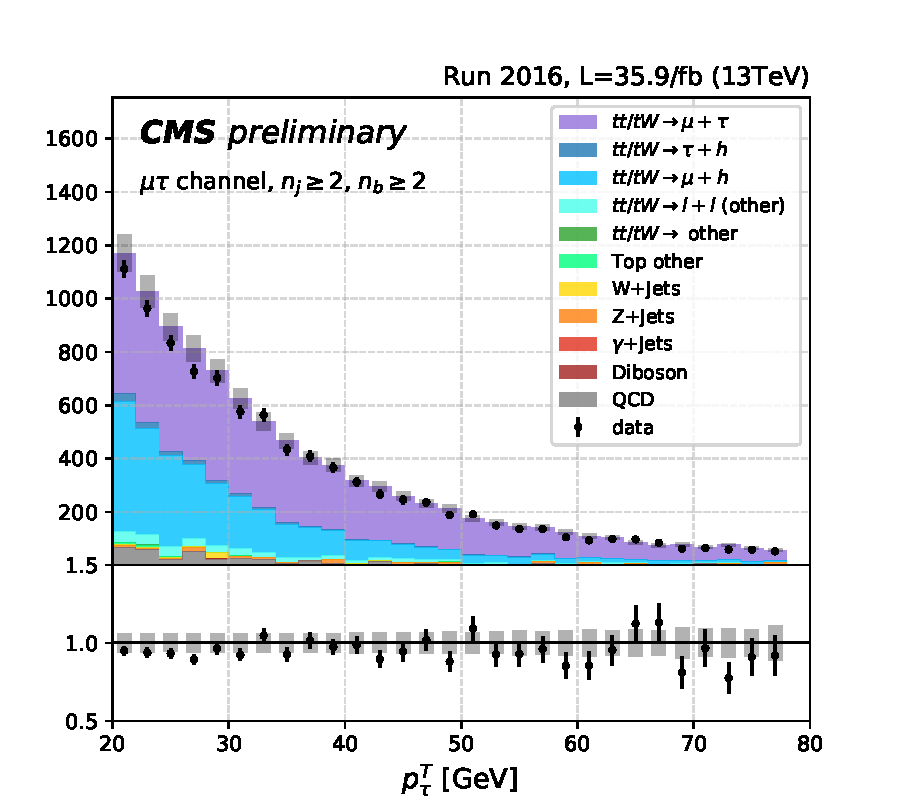
\includegraphics[width=0.24\textwidth]{chapters/Analysis/sectionPlots/figures/kinematics_pickles/mutau/2b/mutau_2b_lepton2_pt.pdf}
        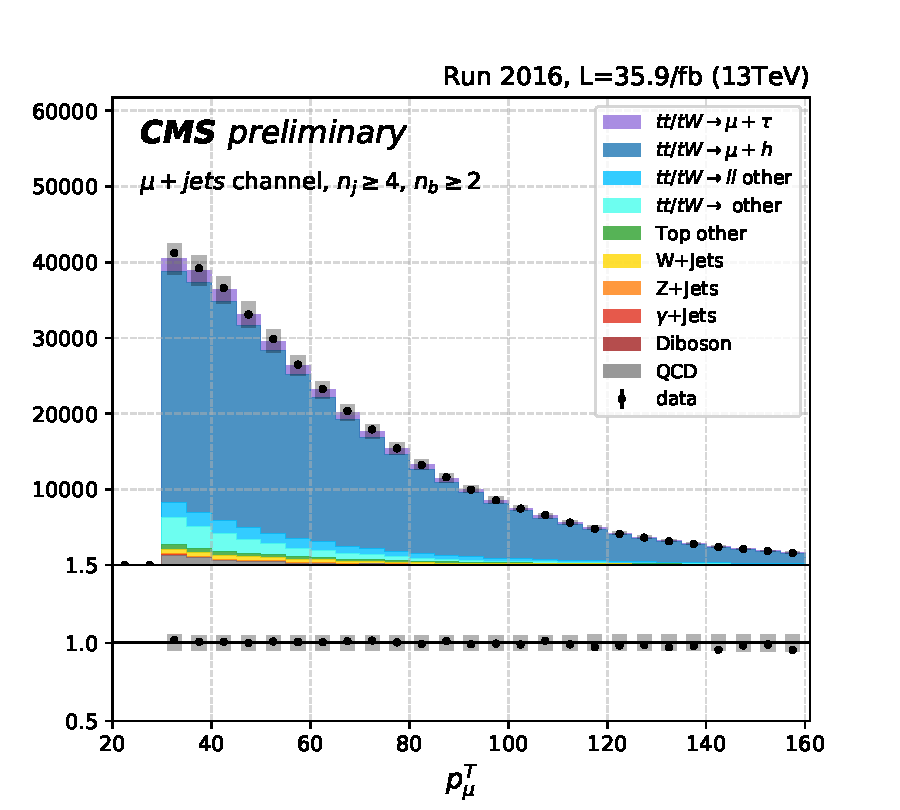
\includegraphics[width=0.24\textwidth]{chapters/Analysis/sectionPlots/figures/kinematics_pickles/mu4j/2b/mu4j_2b_lepton1_pt.pdf}
    \end{center}
    \end{block}
    
    \begin{block}{\smaller \Pe trigger}
    \begin{center}
        \cee \qquad\qquad\qquad\quad \cem \qquad\qquad\qquad\quad \cet \qquad\qquad\qquad\quad \ceh \\
        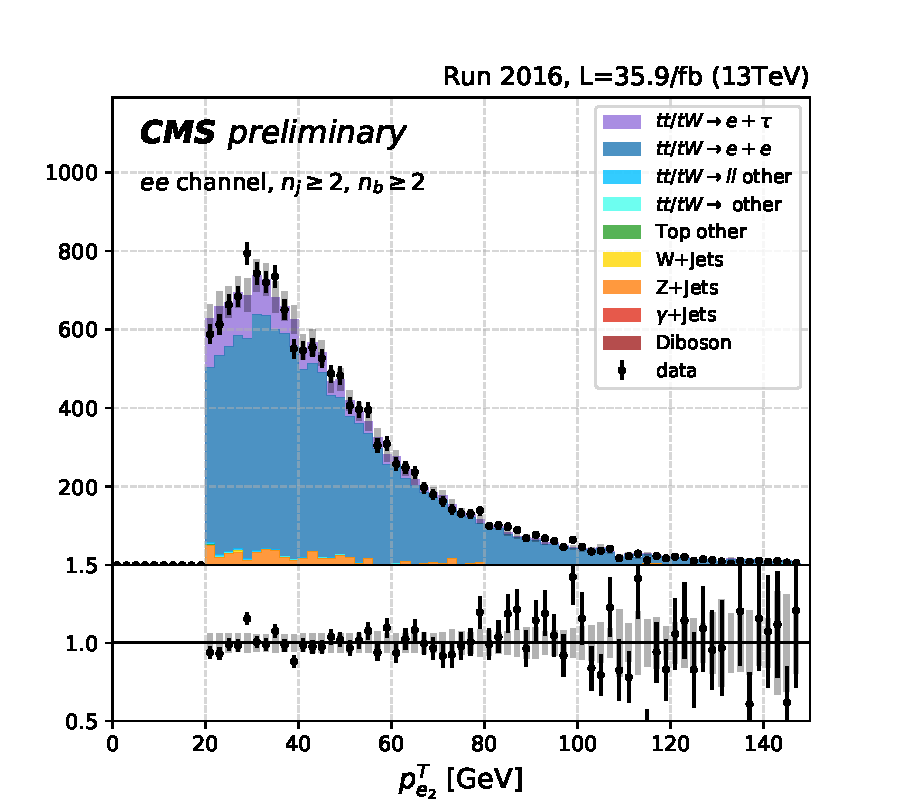
\includegraphics[width=0.24\textwidth]{chapters/Analysis/sectionPlots/figures/kinematics_pickles/ee/2b/ee_2b_lepton2_pt.pdf}
        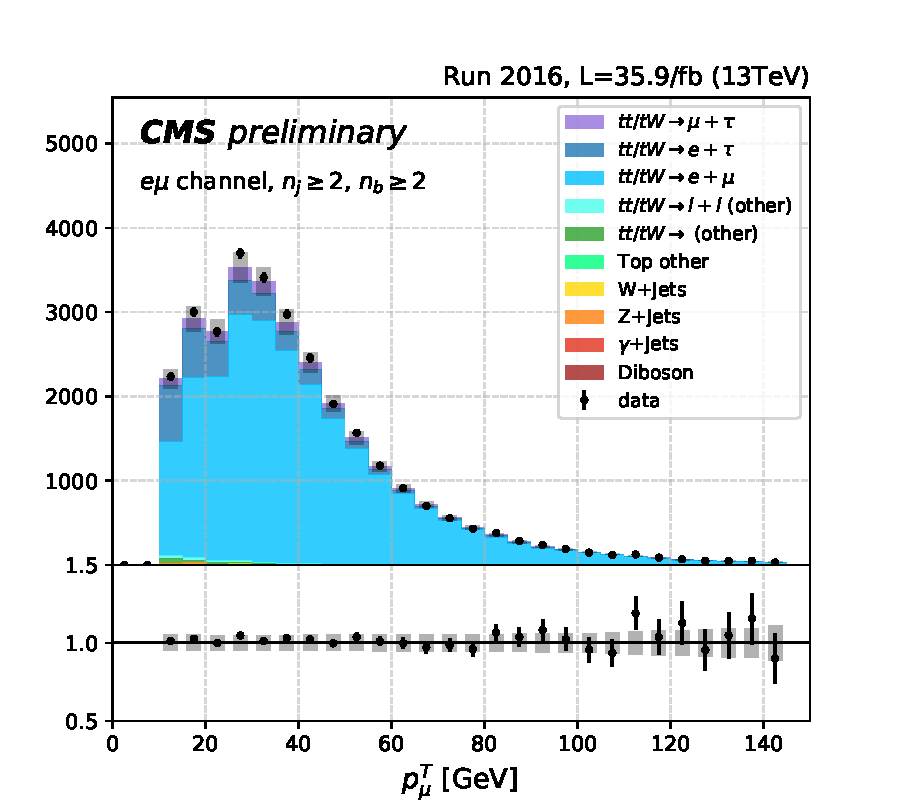
\includegraphics[width=0.24\textwidth]{chapters/Analysis/sectionPlots/figures/kinematics_pickles/emu2/2b/emu2_2b_lepton1_pt.pdf}
        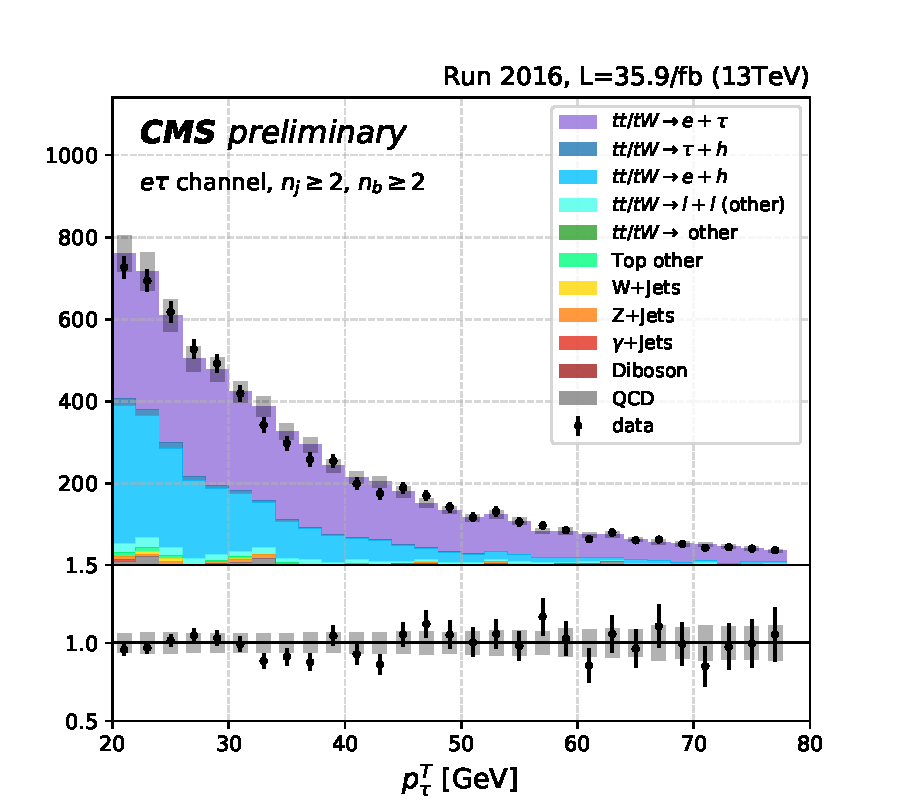
\includegraphics[width=0.24\textwidth]{chapters/Analysis/sectionPlots/figures/kinematics_pickles/etau/2b/etau_2b_lepton2_pt.pdf}
        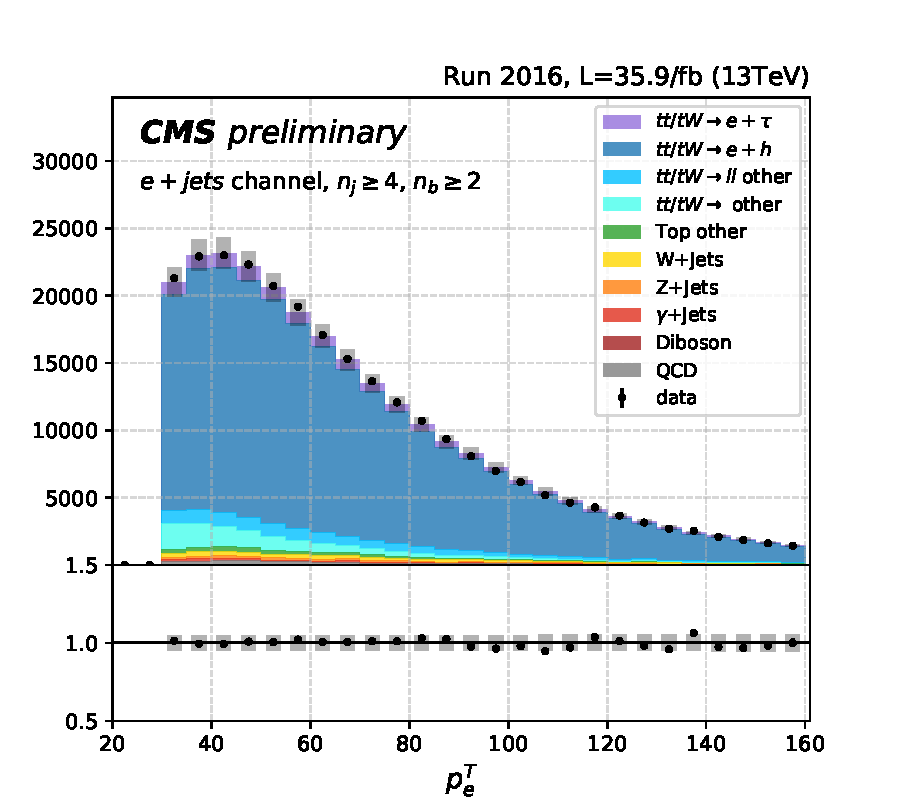
\includegraphics[width=0.24\textwidth]{chapters/Analysis/sectionPlots/figures/kinematics_pickles/e4j/2b/e4j_2b_lepton1_pt.pdf}
    \end{center}
    \end{block}
\end{frame}





% -------------
% new frame
% -------------
\begin{frame}{Extended $n_j$ and $n_b$ categories}
\smaller
    \begin{table}
        \centering
        \setlength{\tabcolsep}{1em}
        \renewcommand{\arraystretch}{1.5}
        \resizebox{0.7\textwidth}{!}{\begin{tabular}{l|c|c|c c|c}

                                    & $N_j = 0$     & $N_j = 1$      & $N_j = 2$                    & \multicolumn{1}{|c|}{$N_j = 3$}   & $N_j \geq 4$ \\
	\hline
    \multirow{2}{*}{$N_\PQb = 0$}   & \cellcolor{NUpurple10}\textcolor{red}{\cet, \cmt,}  & \cellcolor{NUpurple10}\textcolor{red}{\cet, \cmt,} & \multicolumn{2}{c}{\cellcolor{NUpurple10} \textcolor{red}{\cet, \cmt,} }      & \cellcolor{NUpurple10}\\
                                    & \cellcolor{NUpurple10} \textcolor{blue}{\cem}         & \cellcolor{NUpurple10}\textcolor{blue}{\cem}       & \multicolumn{2}{c}{\cellcolor{NUpurple10} \textcolor{orange}{\cem}}& \cellcolor{NUpurple10}\\
	\hline
    \multirow{3}{*}{$N_\PQb = 1$}   &   & \cellcolor{NUpurple10} \textcolor{orange}{\cet, \cmt, \cem } & \cet, \cmt   & \multicolumn{2}{!{\color{OliveGreen}\vrule width 2pt}c}{\cet, \cmt} \\
	\cline{3-6}
                                    & \multicolumn{2}{c|}{} & \multicolumn{3}{c}{ \cee, \cmm, \cem}                                        \\
	\cline{4-6}
                                    & \multicolumn{4}{c|}{} & \ceh, \cmh \\
	\hline

    \multirow{3}{*}{$N_\PQb \geq 2$} & \multicolumn{2}{c|}{} & \cet, \cmt & \multicolumn{2}{!{\color{OliveGreen}\vrule width 2pt}c}{\cet, \cmt} \\
	\cline{4-6}
                                    & \multicolumn{2}{c|}{} & \multicolumn{3}{c}{$\cee, \cmm, \cem$}                                        \\
	\cline{4-6}
                                    & \multicolumn{4}{c|}{} & \ceh, \cmh \\
	\hline
\end{tabular}}
    \end{table}

    \begin{block}{extended $n_j$ and $n_b$ categories in shape analysis}
    \begin{itemize}
        \item \textcolor{red}{Enriched with $\PZ \to \PGtl \PGth$ to constrain \PGth systematics.}
        extra cuts on $m_{\ell \PGth}$, $\Delta\phi(\ell,\PGth)$, $\mT^{\ell,MET}$ to enhance \zjets over \wjets.
        \item \textcolor{OliveGreen}{Bin $n_j$ finer in \cet and \cmt to better discriminate $\PW\to \PGth$ and $\PW\to jj$}
        \item \textcolor{blue}{Add \WW events}
        \item \textcolor{orange}{Add more \ttbar events}
    \end{itemize}
    \end{block}
\end{frame}


% -------------
% new frame
% -------------
\begin{frame}{}

    \begin{tcolorbox}[colframe=red,colback=white]{$\PZ\to \PGtl \PGth$}
    \smaller
        \begin{center}
        \color{red}
        $\cet: n_j=0, n_b=0$ \hspace{0.12\textwidth} $n_j=1, n_b=0$ \hspace{0.12\textwidth} $n_j\geq2, n_b=0$ \\
        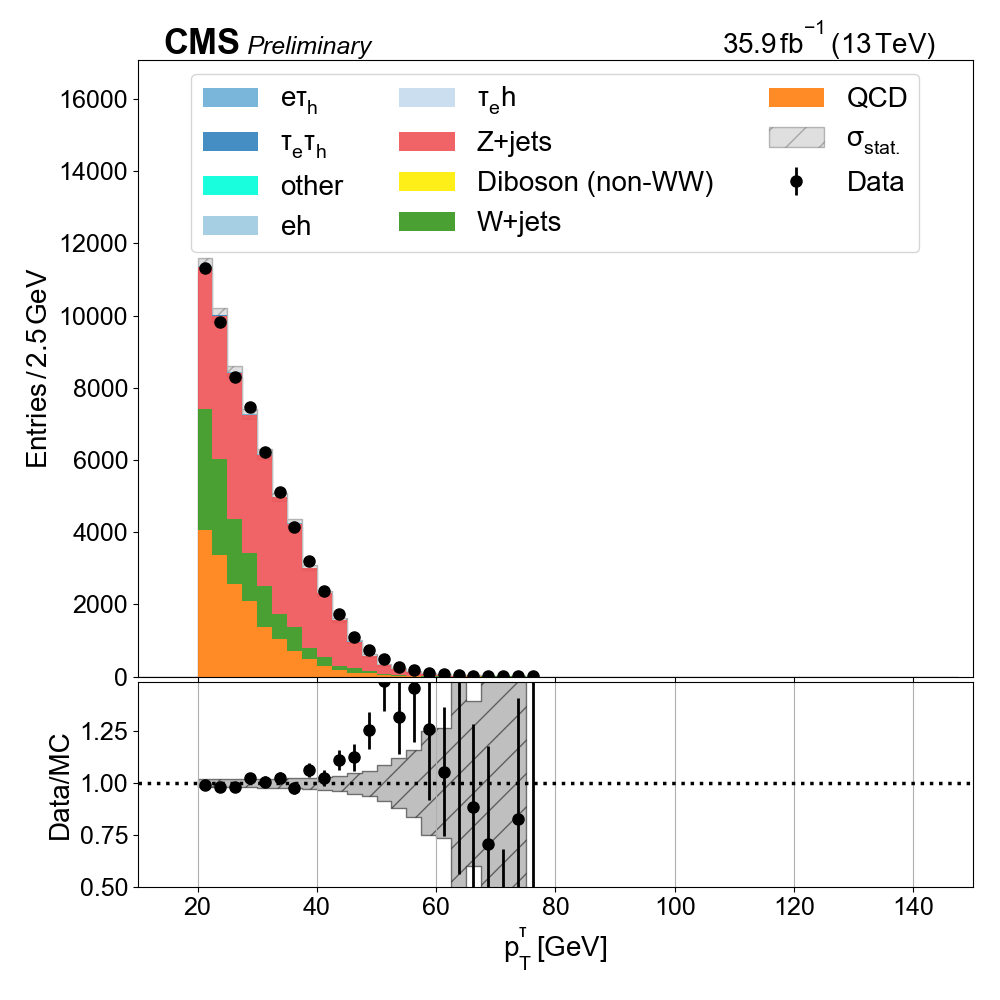
\includegraphics[width=0.3\textwidth]{chapters/Analysis/sectionPlots/figures/data_mc_overlays/etau_2016_cat_eq0_eq0_signal_linear_lepton_lepton2_pt.png}
        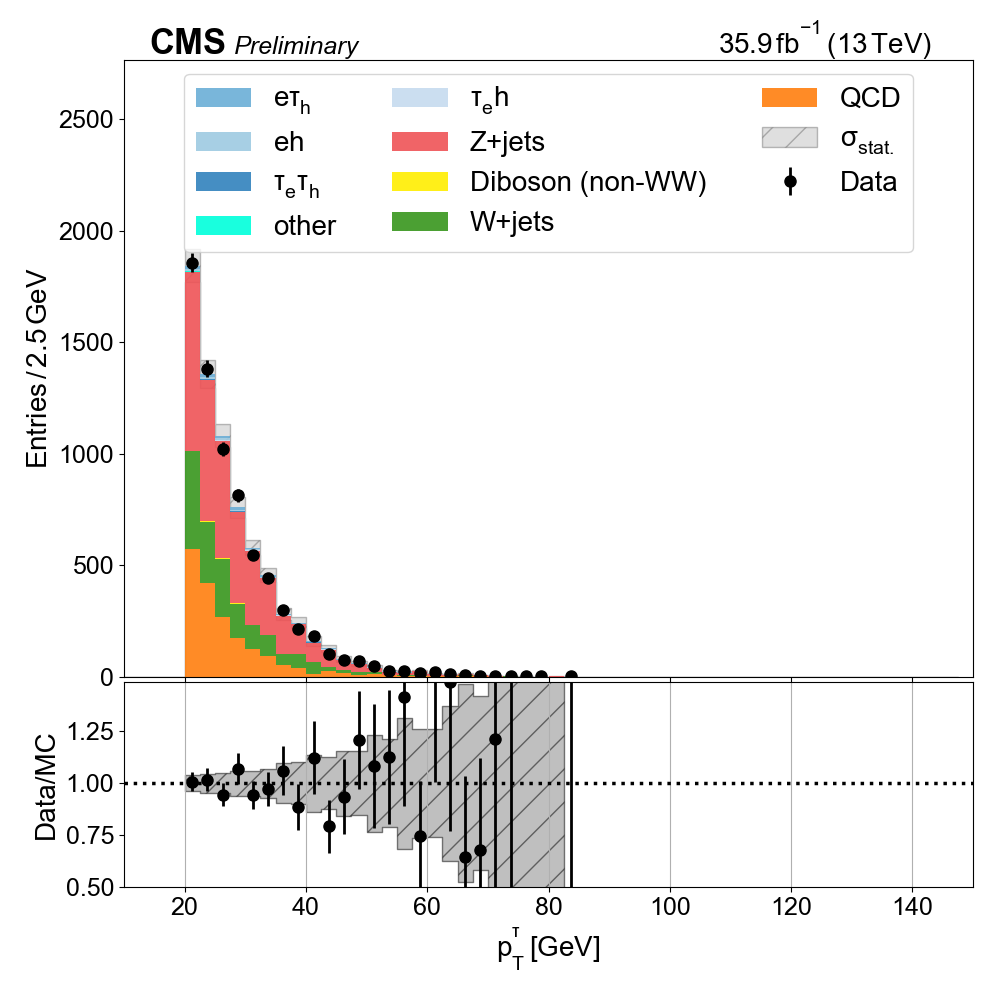
\includegraphics[width=0.3\textwidth]{chapters/Analysis/sectionPlots/figures/data_mc_overlays/etau_2016_cat_eq1_eq0_signal_linear_lepton_lepton2_pt.png}
        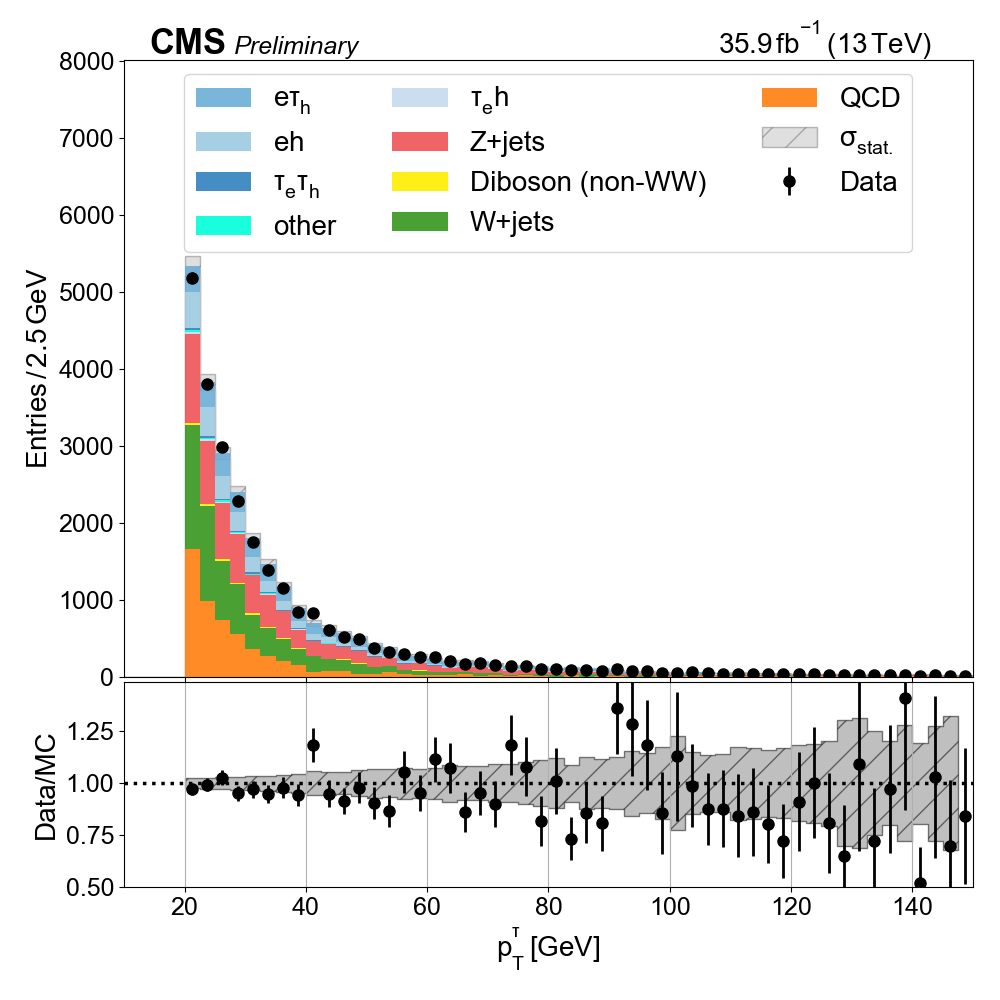
\includegraphics[width=0.3\textwidth]{chapters/Analysis/sectionPlots/figures/data_mc_overlays/etau_2016_cat_gt2_eq0_signal_linear_lepton_lepton2_pt.png} \\
        $\cmt: n_j=0, n_b=0$ \hspace{0.12\textwidth} $n_j=1, n_b=0$ \hspace{0.12\textwidth} $n_j\geq2, n_b=0$ \\
        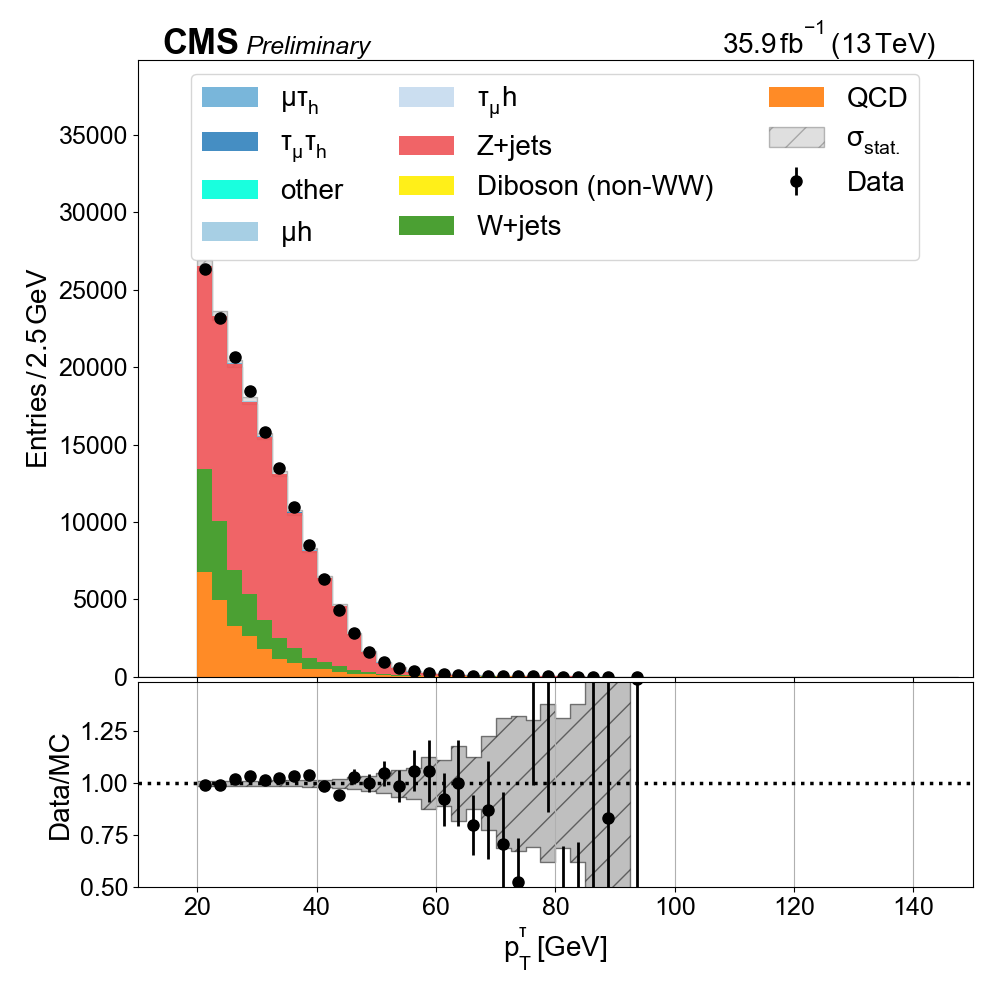
\includegraphics[width=0.3\textwidth]{chapters/Analysis/sectionPlots/figures/data_mc_overlays/mutau_2016_cat_eq0_eq0_signal_linear_lepton_lepton2_pt.png}
        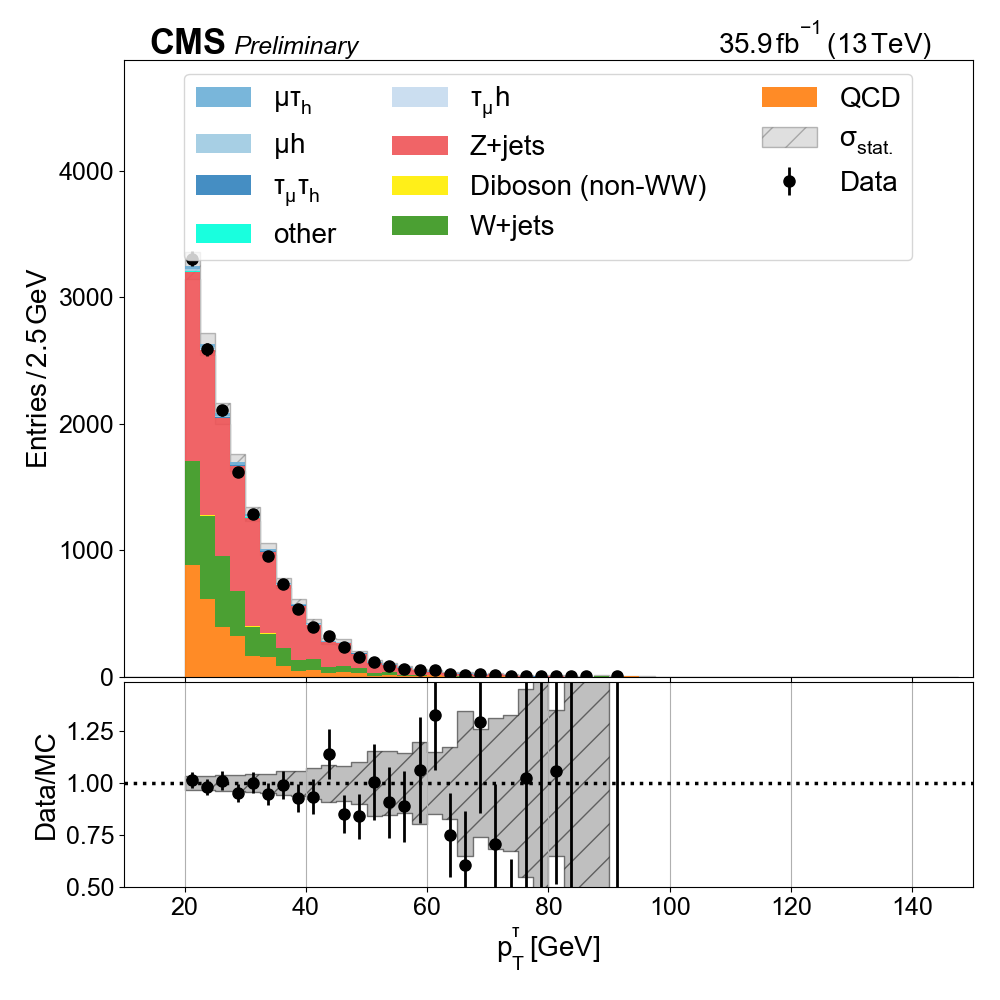
\includegraphics[width=0.3\textwidth]{chapters/Analysis/sectionPlots/figures/data_mc_overlays/mutau_2016_cat_eq1_eq0_signal_linear_lepton_lepton2_pt.png}
        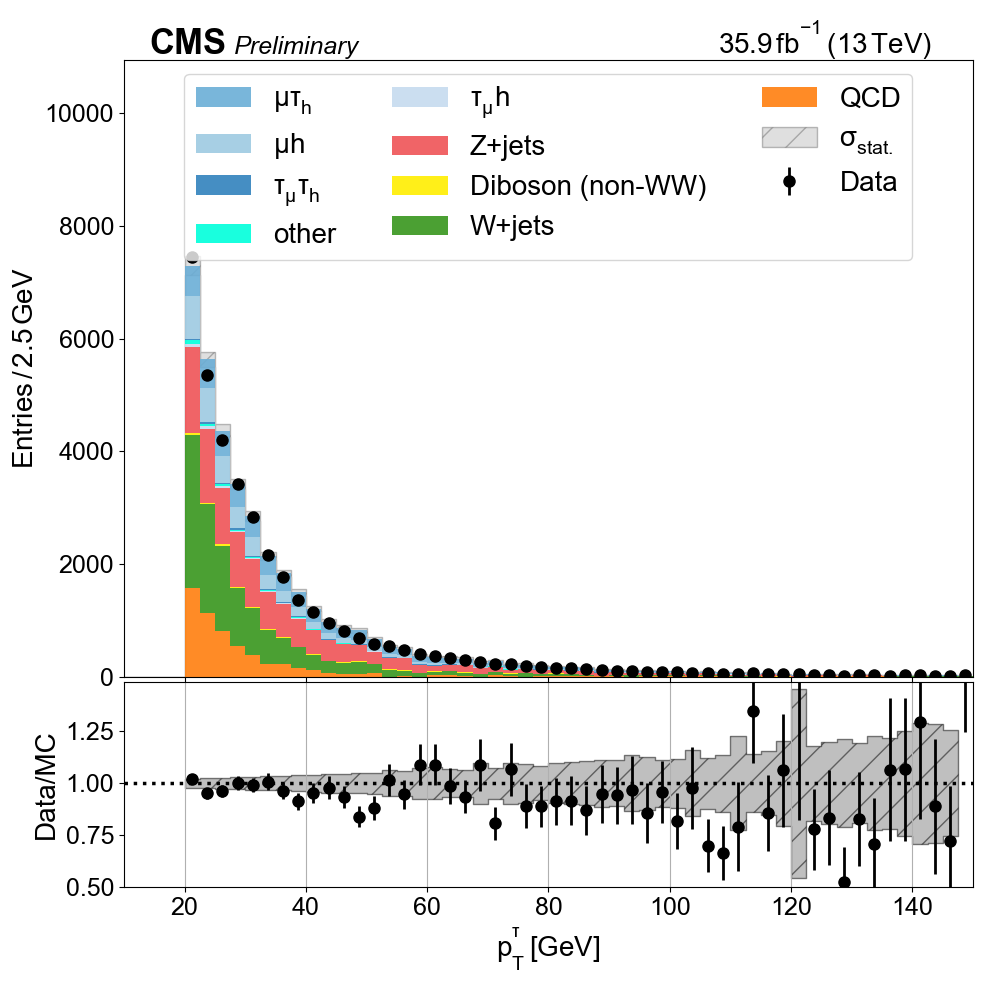
\includegraphics[width=0.3\textwidth]{chapters/Analysis/sectionPlots/figures/data_mc_overlays/mutau_2016_cat_gt2_eq0_signal_linear_lepton_lepton2_pt.png}        
        \end{center}
    \end{tcolorbox}
\end{frame}

% -------------
% new frame
% -------------
\begin{frame}{}
    \begin{columns}
        \column{0.33\textwidth}
        \begin{tcolorbox}[colframe=OliveGreen,colback=white]{finer $n_j$ binning}
            \begin{center}
            \color{OliveGreen}
            \smaller \smaller
            $n_j$ distribution of \cet\\
            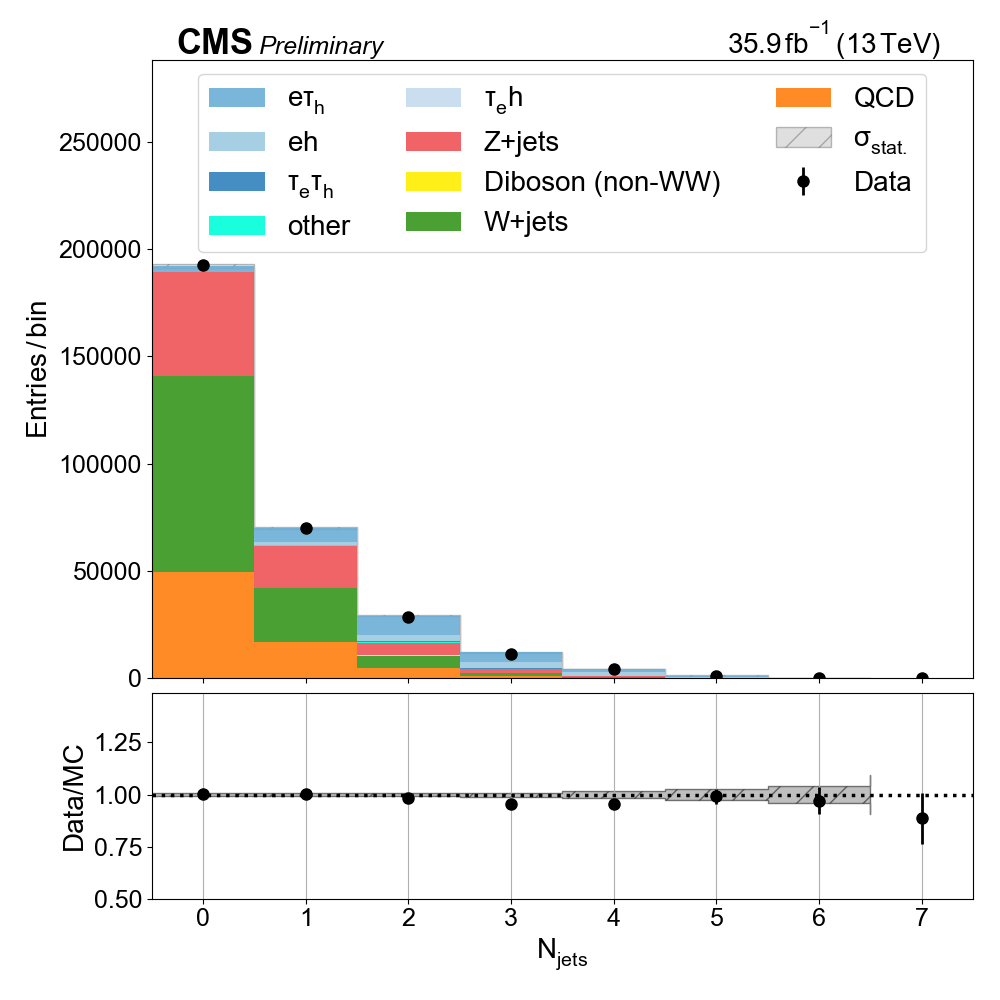
\includegraphics[width=\textwidth]{chapters/Analysis/sectionPlots/figures/data_mc_overlays/etau_2016_inclusive_linear_jet_n_jets.png}
            \end{center}
        \end{tcolorbox}
        
        \column{0.6\textwidth}
        \begin{tcolorbox}[colframe=blue,colback=white]{$\WW \to \Pe \PGm$}
            \begin{center}
            \color{blue}
            \smaller \smaller
            $\cem: n_j=0, n_b=0$ \hspace{0.1\textwidth} $n_j=1, n_b=0$  \\
            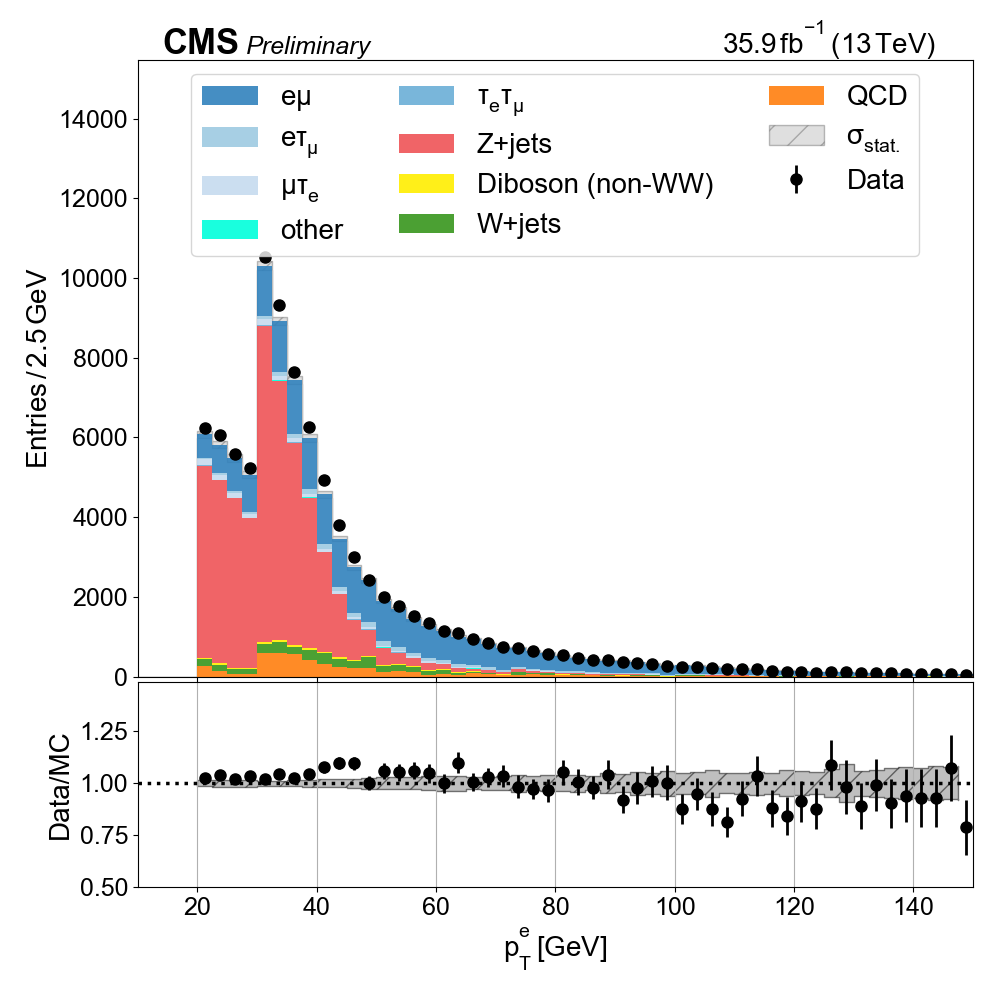
\includegraphics[width=0.48\textwidth]{chapters/Analysis/sectionPlots/figures/data_mc_overlays/emu_2016_cat_eq0_eq0_a_signal_linear_lepton_lepton2_pt.png}
            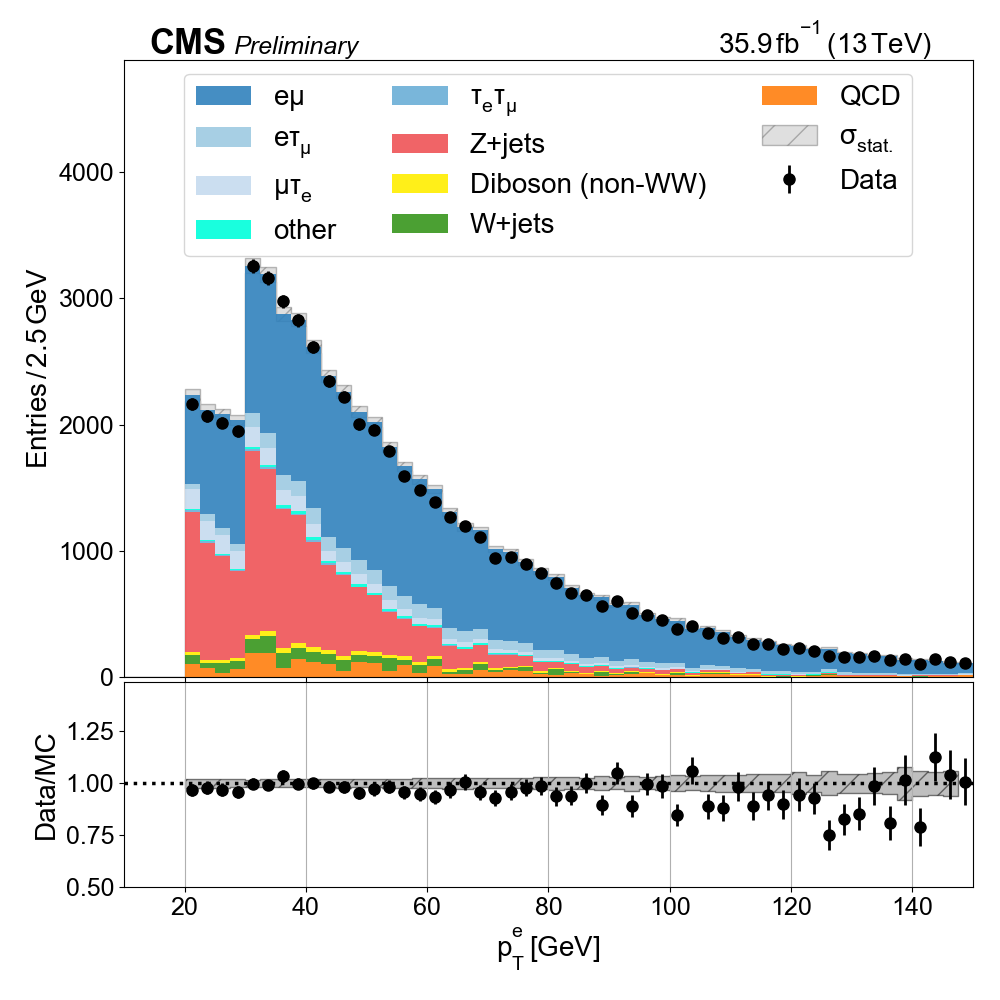
\includegraphics[width=0.48\textwidth]{chapters/Analysis/sectionPlots/figures/data_mc_overlays/emu_2016_cat_eq1_eq0_a_signal_linear_lepton_lepton2_pt.png}
            \end{center}
        \end{tcolorbox}
    \end{columns}
    
    
    \begin{tcolorbox}[colframe=orange,colback=white]{$\ttbar$ extra}
        \begin{center}
        \color{orange}
        \smaller \smaller
        $\cet: n_j=1, n_b=1$ \hspace{0.04\textwidth} $\cmt: n_j=1, n_b=1$ \hspace{0.04\textwidth} $\cem: n_j=1, n_b=1$ \hspace{0.04\textwidth} $\cem: n_j\geq2, n_b=0$ \\
        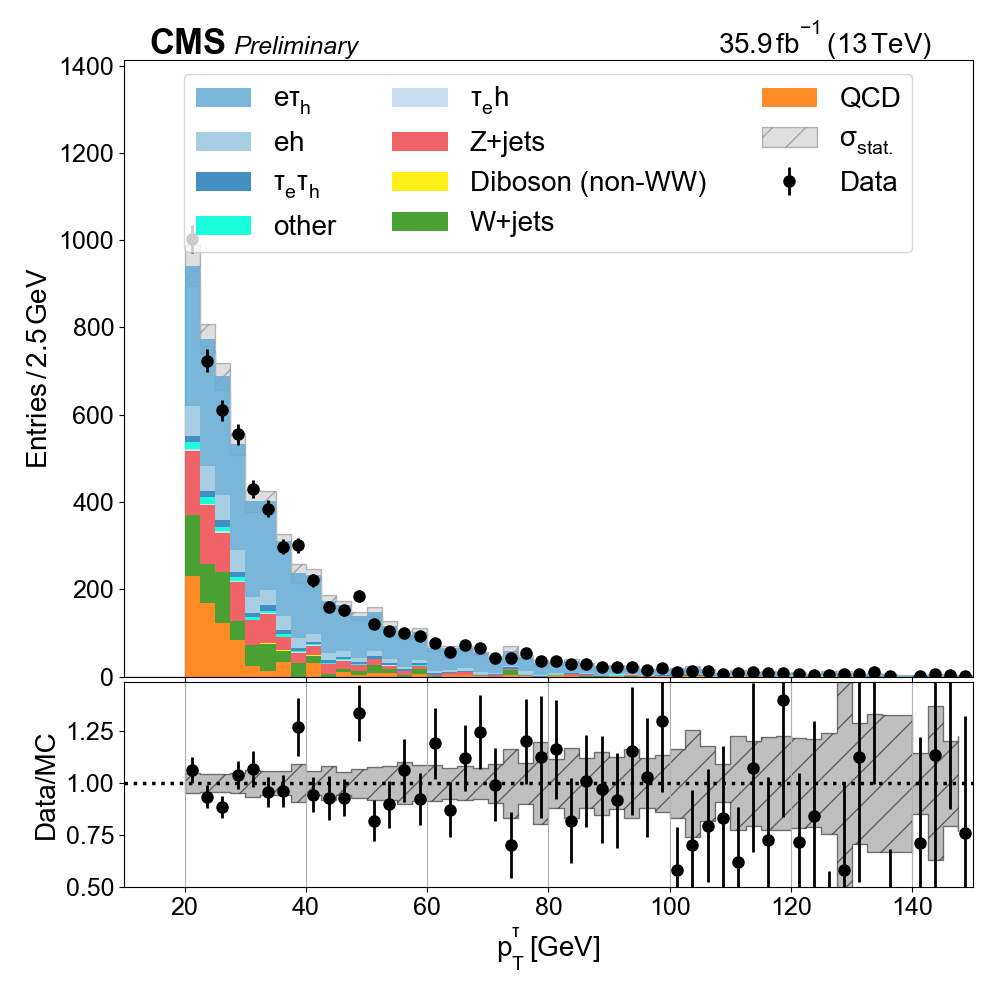
\includegraphics[width=0.24\textwidth]{chapters/Analysis/sectionPlots/figures/data_mc_overlays/etau_2016_cat_eq1_eq1_signal_linear_lepton_lepton2_pt.png}
        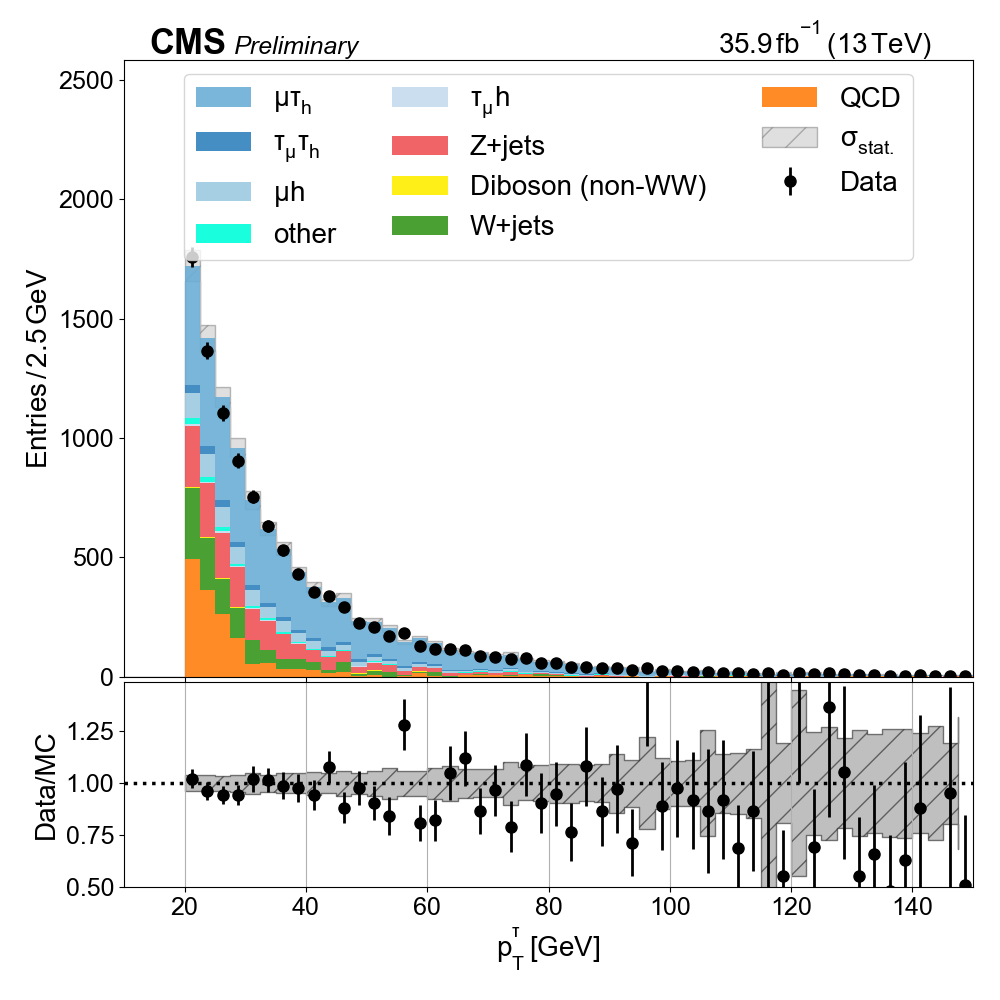
\includegraphics[width=0.24\textwidth]{chapters/Analysis/sectionPlots/figures/data_mc_overlays/mutau_2016_cat_eq1_eq1_signal_linear_lepton_lepton2_pt.png}
        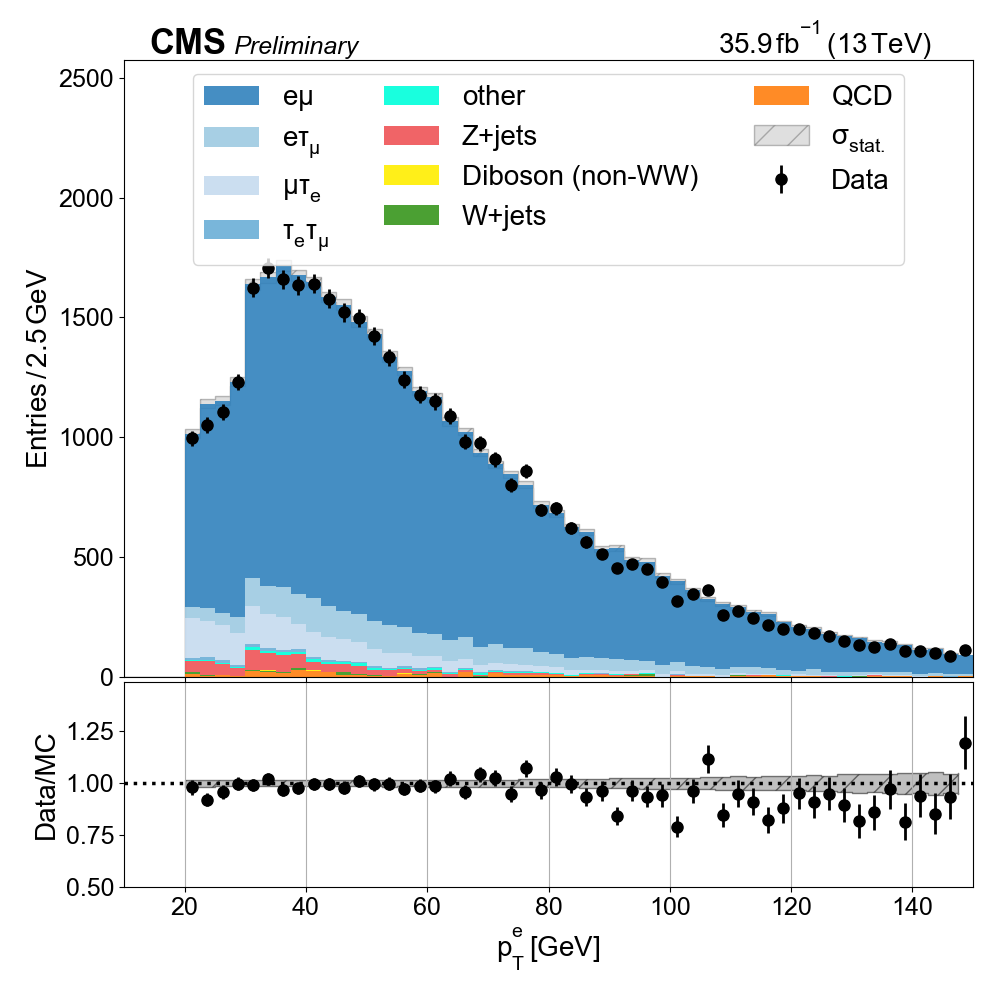
\includegraphics[width=0.24\textwidth]{chapters/Analysis/sectionPlots/figures/data_mc_overlays/emu_2016_cat_eq1_eq1_a_signal_linear_lepton_lepton2_pt.png}
        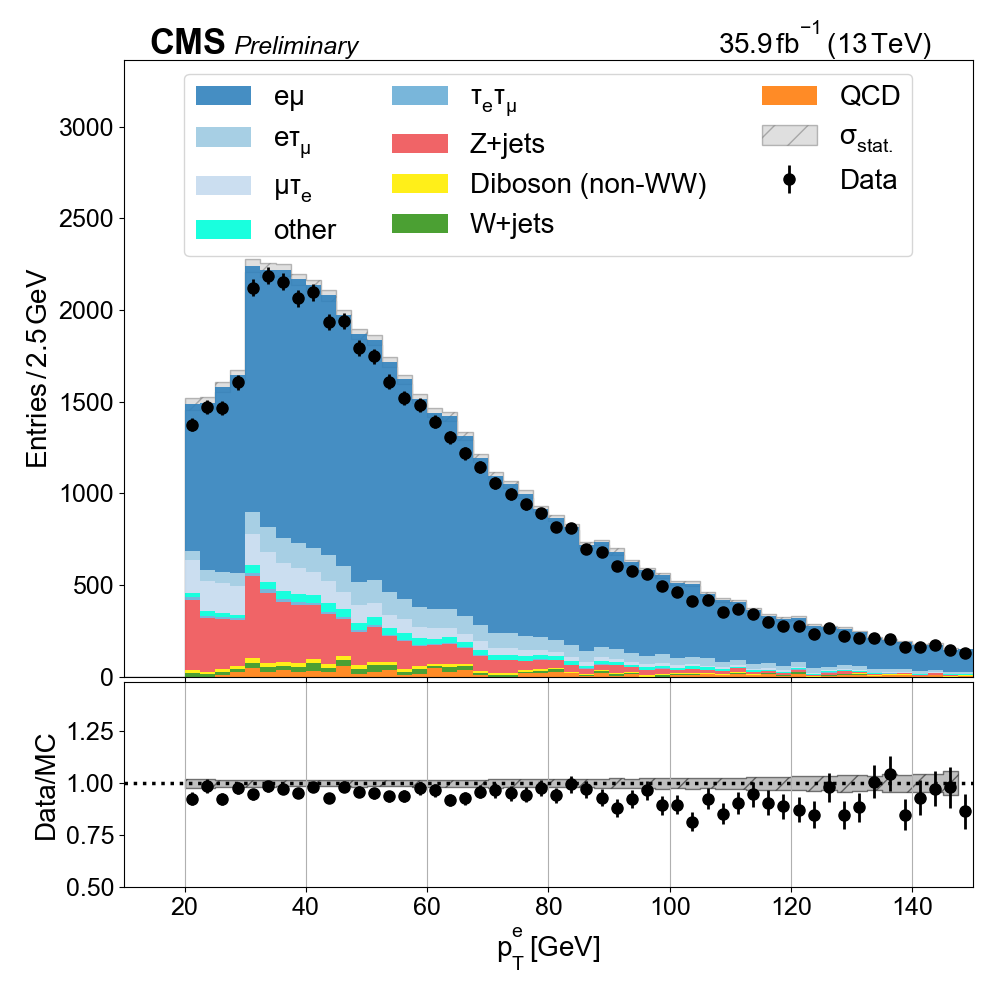
\includegraphics[width=0.24\textwidth]{chapters/Analysis/sectionPlots/figures/data_mc_overlays/emu_2016_cat_gt2_eq0_signal_linear_lepton_lepton2_pt.png}
        
        \end{center}
    \end{tcolorbox}
    
\end{frame}





\subsection{Calibrations}

% -------------
% new frame
% -------------
\begin{frame}{Corrections and calibrations}
\smaller
    \begin{columns}

        % add column
        \column{0.4\textwidth}
        \begin{block}{Generator}
            \begin{itemize}
                \item pile-up
                \item top \pt
                \item \PZ \pt
                \item \WW \pt
            \end{itemize}
        \end{block}
        
        \begin{block}{Trigger}
            \begin{itemize}
                \item single muon trigger efficiency
                \item \alert{single electron trigger efficiency}
                \item electron L1T prefiring correction
            \end{itemize}
        \end{block}
        
        
        % add column
        \column{0.4\textwidth}
        \begin{block}{Objects}
            \begin{itemize}
                \item \Pe
                \begin{itemize}
                \smaller
                    \item energy scale and resolution
                    \item reconstruction efficiency
                    \item isolation efficiency
                \end{itemize}
                \item \PGm: 
                \begin{itemize}
                \smaller
                    \item energy scale
                    \item identification efficiency
                    \item isolation efficiency
                \end{itemize}
                
                \item \PGth: 
                \begin{itemize}
                \smaller
                    \item energy scale
                    \item identification efficiency
                    \item \alert{mis-identification rate}
                \end{itemize}
                \item jet: 
                \begin{itemize}
                \smaller
                    \item energy scale and resolution
                \end{itemize}
                \item b tag: 
                \begin{itemize}
                \smaller
                    \item tag efficiency
                    \item mis-tag rate
                \end{itemize}
            \end{itemize}
        \end{block}
        
    \end{columns}
\end{frame}



% -------------
% new frame
% -------------
\begin{frame}{Single electron trigger efficiency}
\smaller \smaller
    \begin{columns}
        \column{0.6\textwidth}
        \begin{itemize}
            \item Perform a customized measurement of scale factors accounting for the difference of the single electron trigger efficiency in data and simulation.
            \item Use tag-prob approach:
            \begin{itemize} 
            \smaller
                \item electron: same as object selection;
                \item tagged electron: $\pt > 30\GeV$ triggered;
                \item \alert{two opposite electrons (at least one tagged);}
                \item $60<m_{\cee}<120\GeV$;
                \item for each tagged electron, the other electron become prob for measurement.
            \end{itemize}
            \item Trigger efficiency is defined as 
            $$ \epsilon (\pt, \eta) = \frac{ N_{\rm passing} (\pt, \eta) } {  N_{\rm total} (\pt, \eta) } $$.
            \item Scale factor to measure is the ratio of $\epsilon (\pt, \eta)$ between data and MC 
            $$ SF (\pt, \eta) = \frac{\epsilon_{\rm{Data}} (\pt, \eta) }{\epsilon_{\rm{MC}} (\pt, \eta) }. $$
            \item Split into BCDEF and GH periods. (Si-strip problem)
            \item Systematic uncertainties are estimated by shifting \pt of tags and probs.
        \end{itemize}
        
        \column{0.35\textwidth}
        \begin{block}{}
            \centering
            dominated by \zjets
            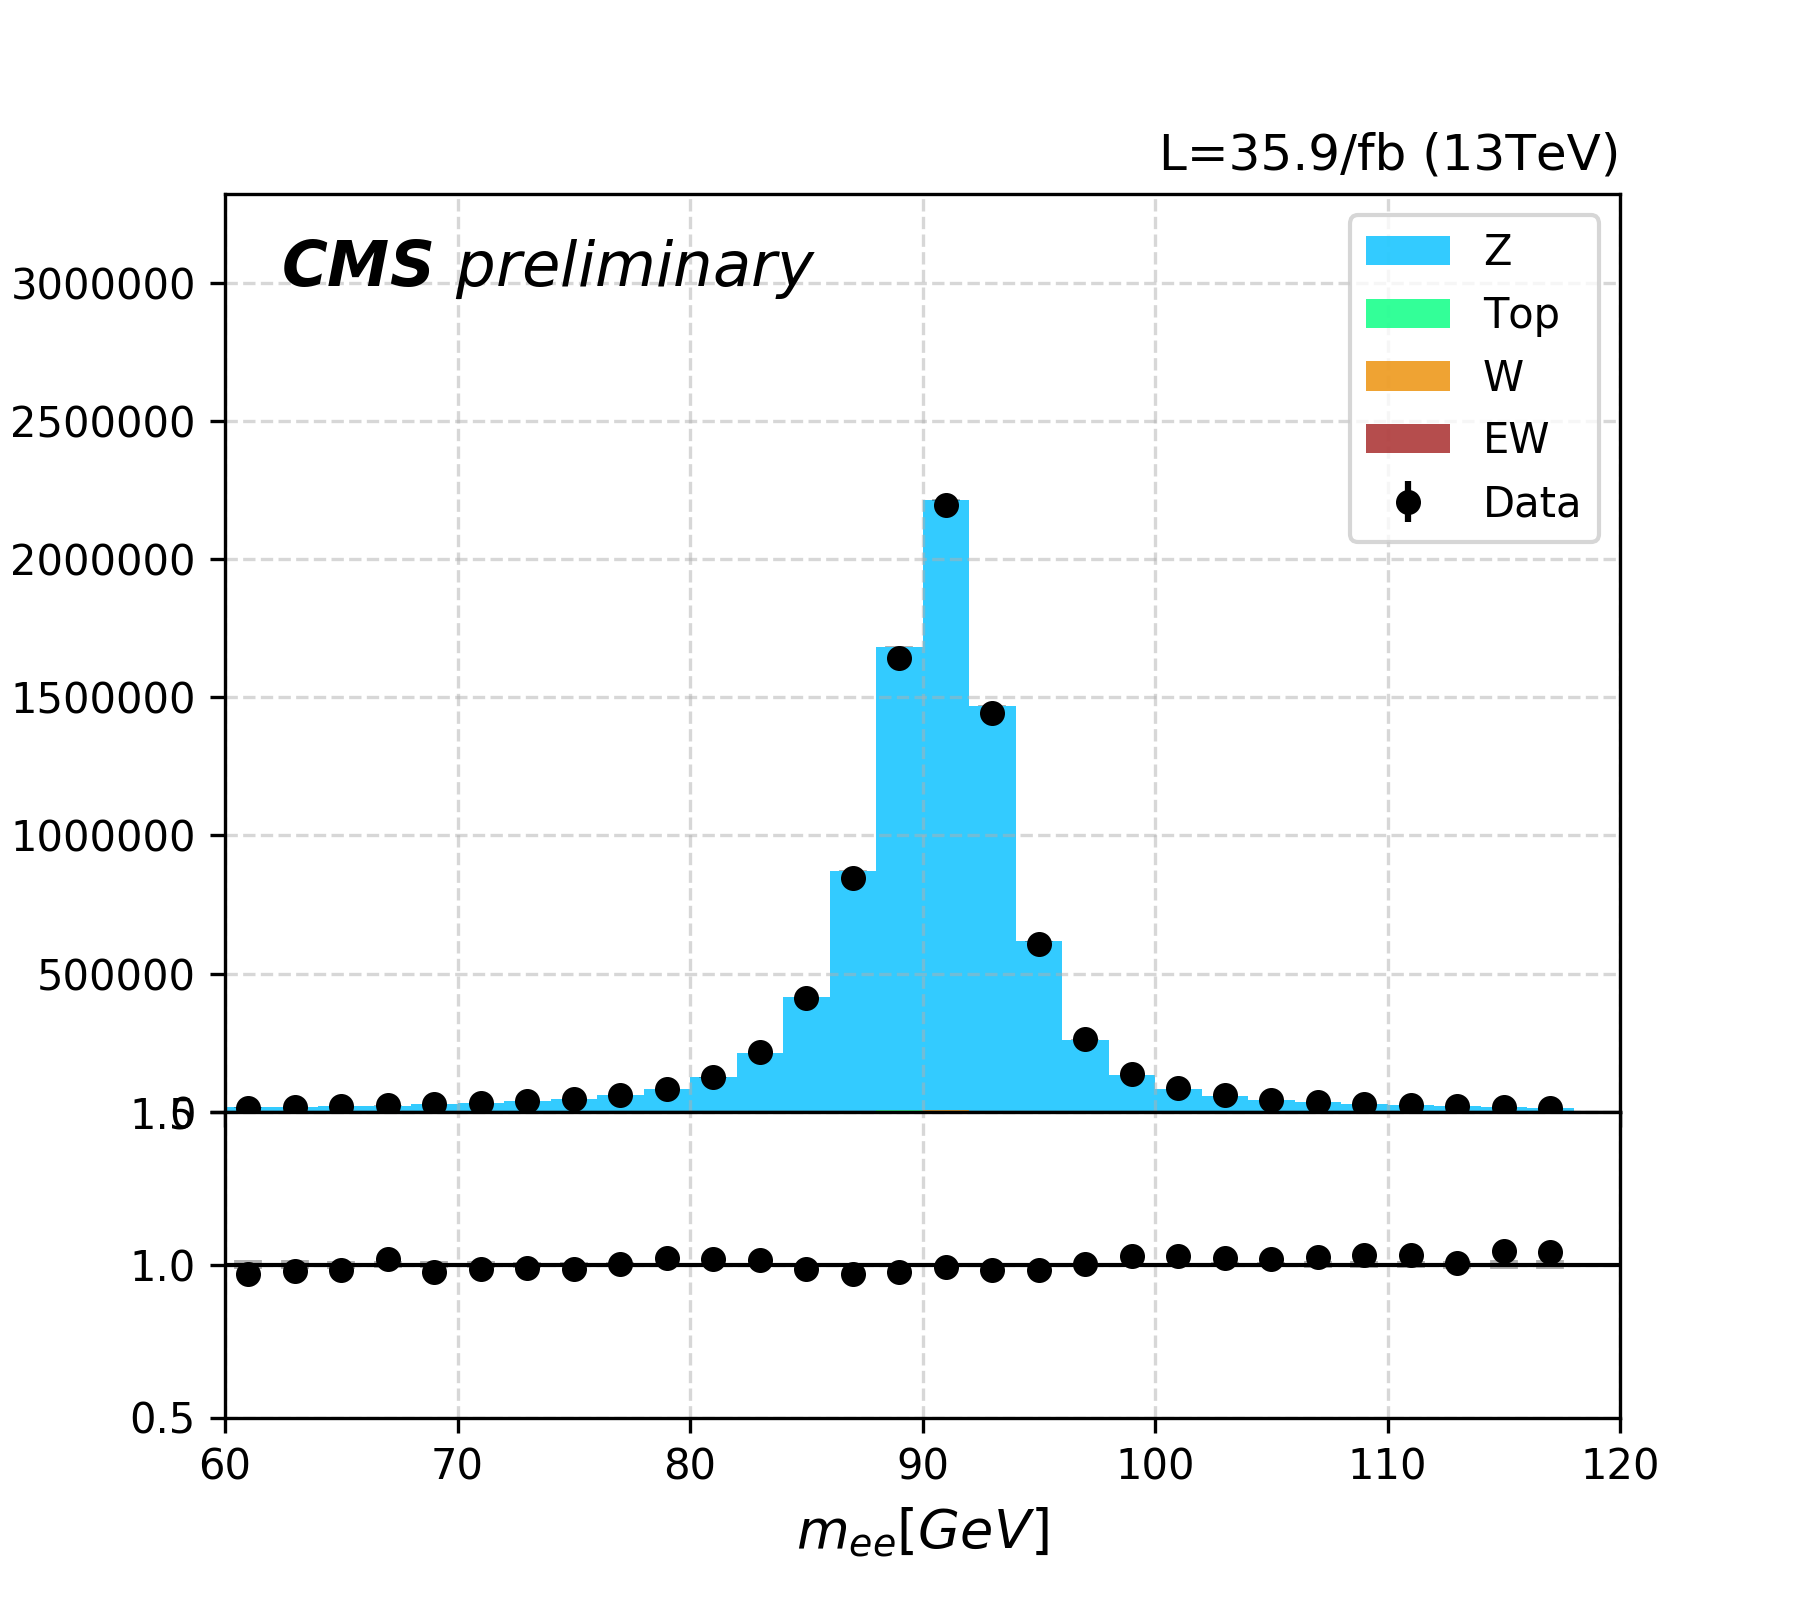
\includegraphics[width=\textwidth]{chapters/Analysis/sectionCalibration/figures/eTrigger/dileptonMass_tag30.png}
        \end{block}
        \begin{center}
            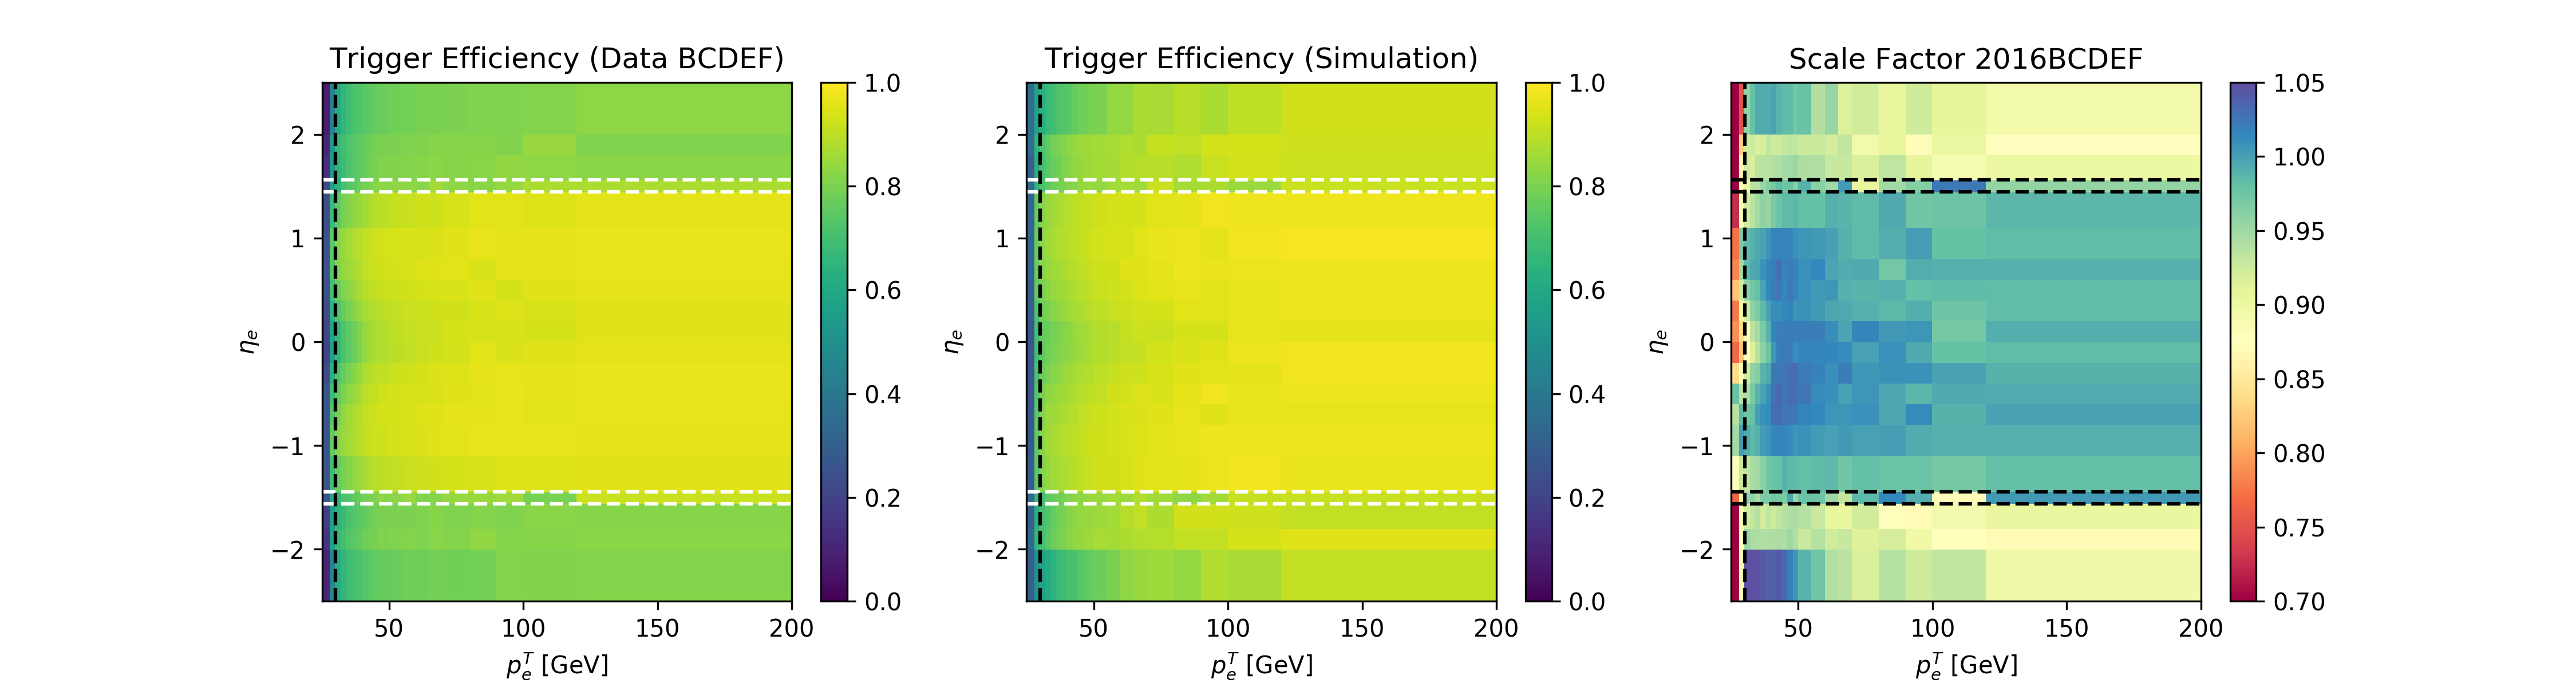
\includegraphics[width=0.49\textwidth, trim=24cm 0 3.7cm 0, clip]{chapters/Analysis/sectionCalibration/figures/eTrigger/eff2d_BCDEF.png}
            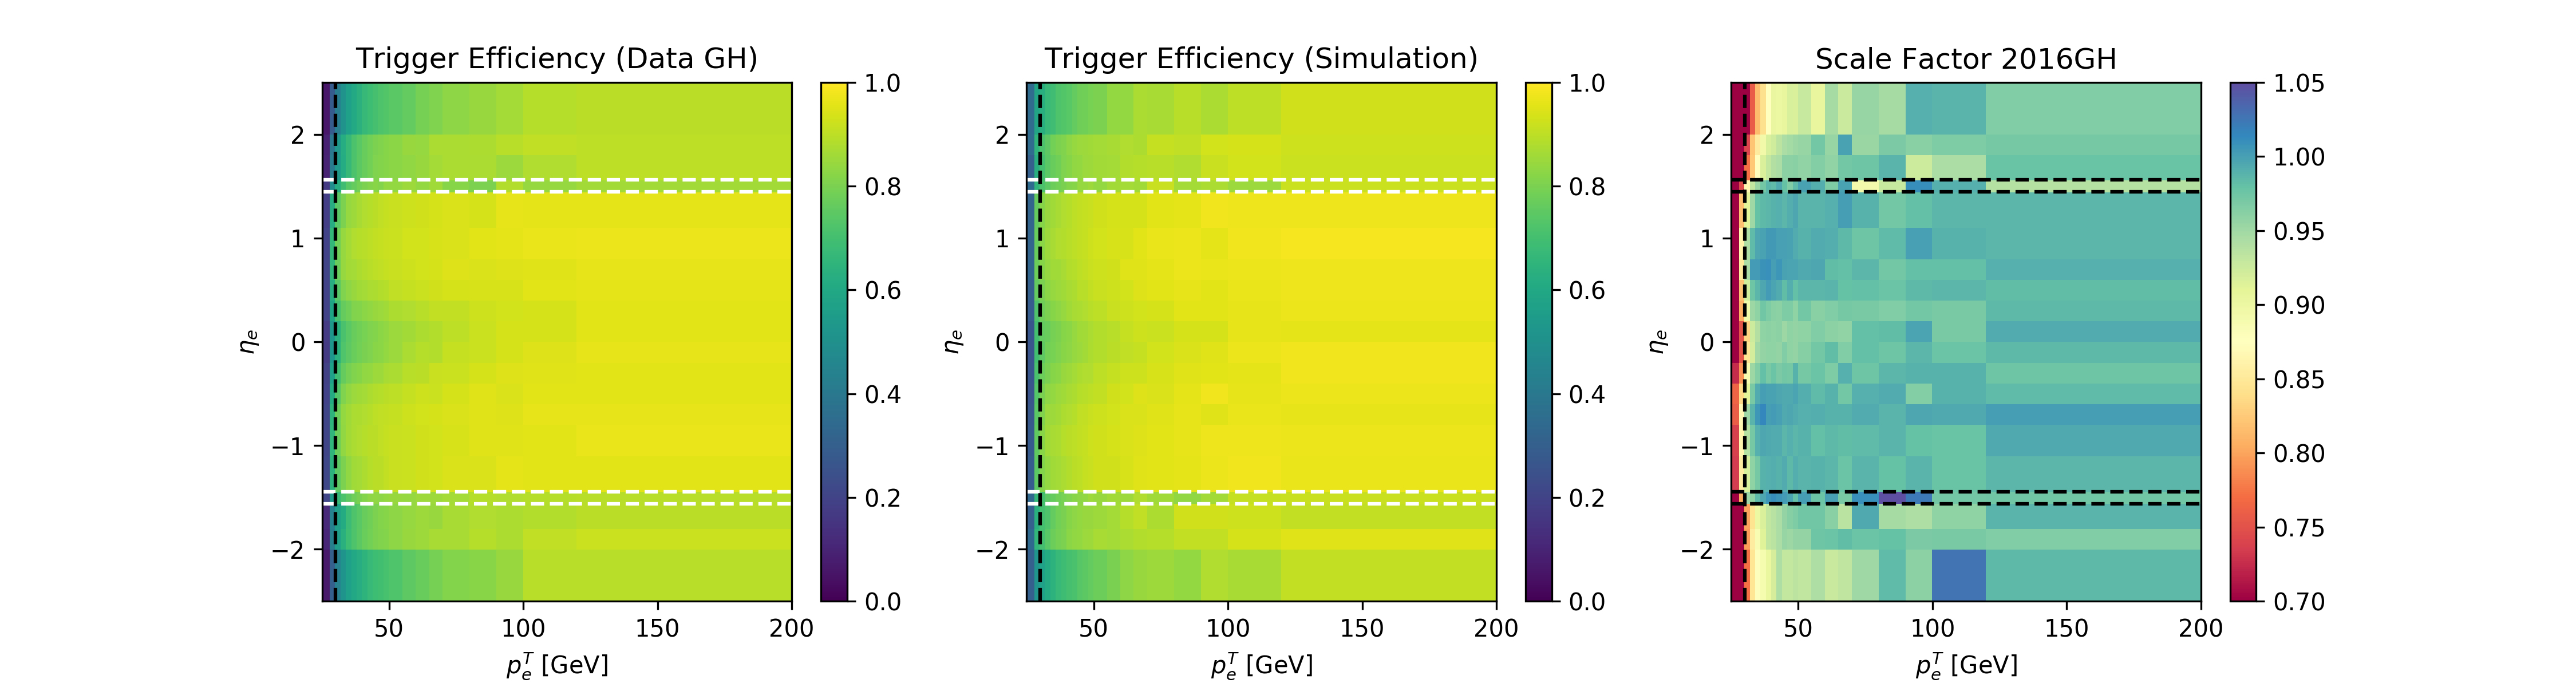
\includegraphics[width=0.49\textwidth, trim=24cm 0 3.7cm 0, clip]{chapters/Analysis/sectionCalibration/figures/eTrigger/eff2d_GH.png}
        \end{center}
    
    \end{columns}
    

\end{frame}



% -------------
% new frame
% -------------
\begin{frame}{$j\to \PGth$ mis-identification}
\smaller \smaller
    \begin{columns}
        \column{0.35\textwidth}
        \begin{block}{\smaller \cmt with $n_j\geq2$, $n_b=1$}
        \centering
            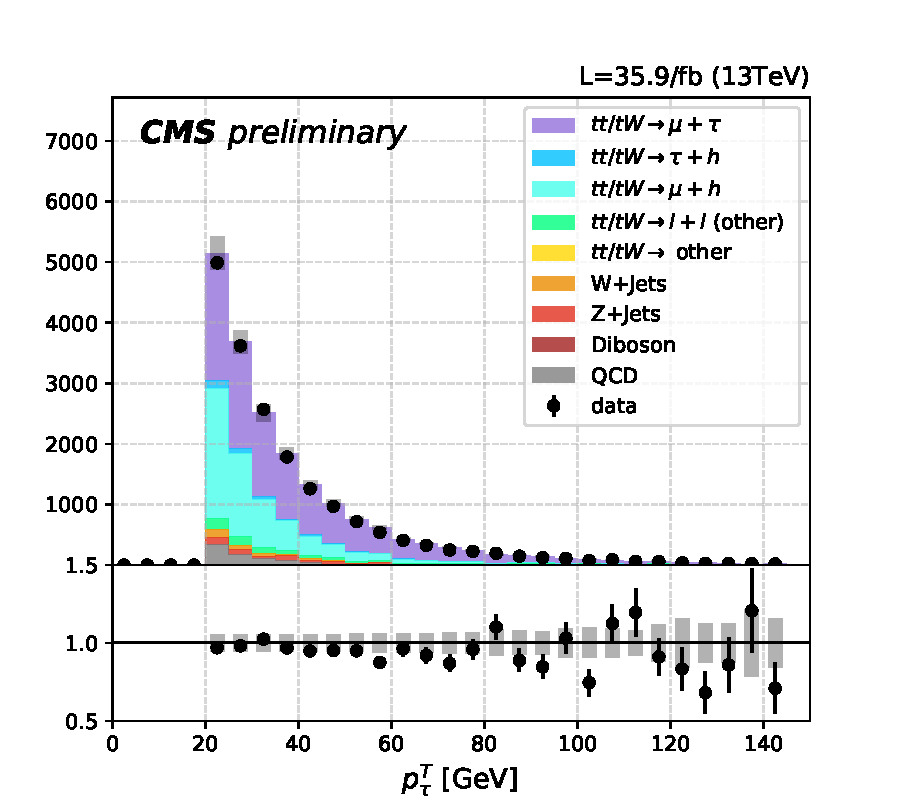
\includegraphics[width=\textwidth]{slides/figures/mutau_1b_lepton2_pt.pdf}
            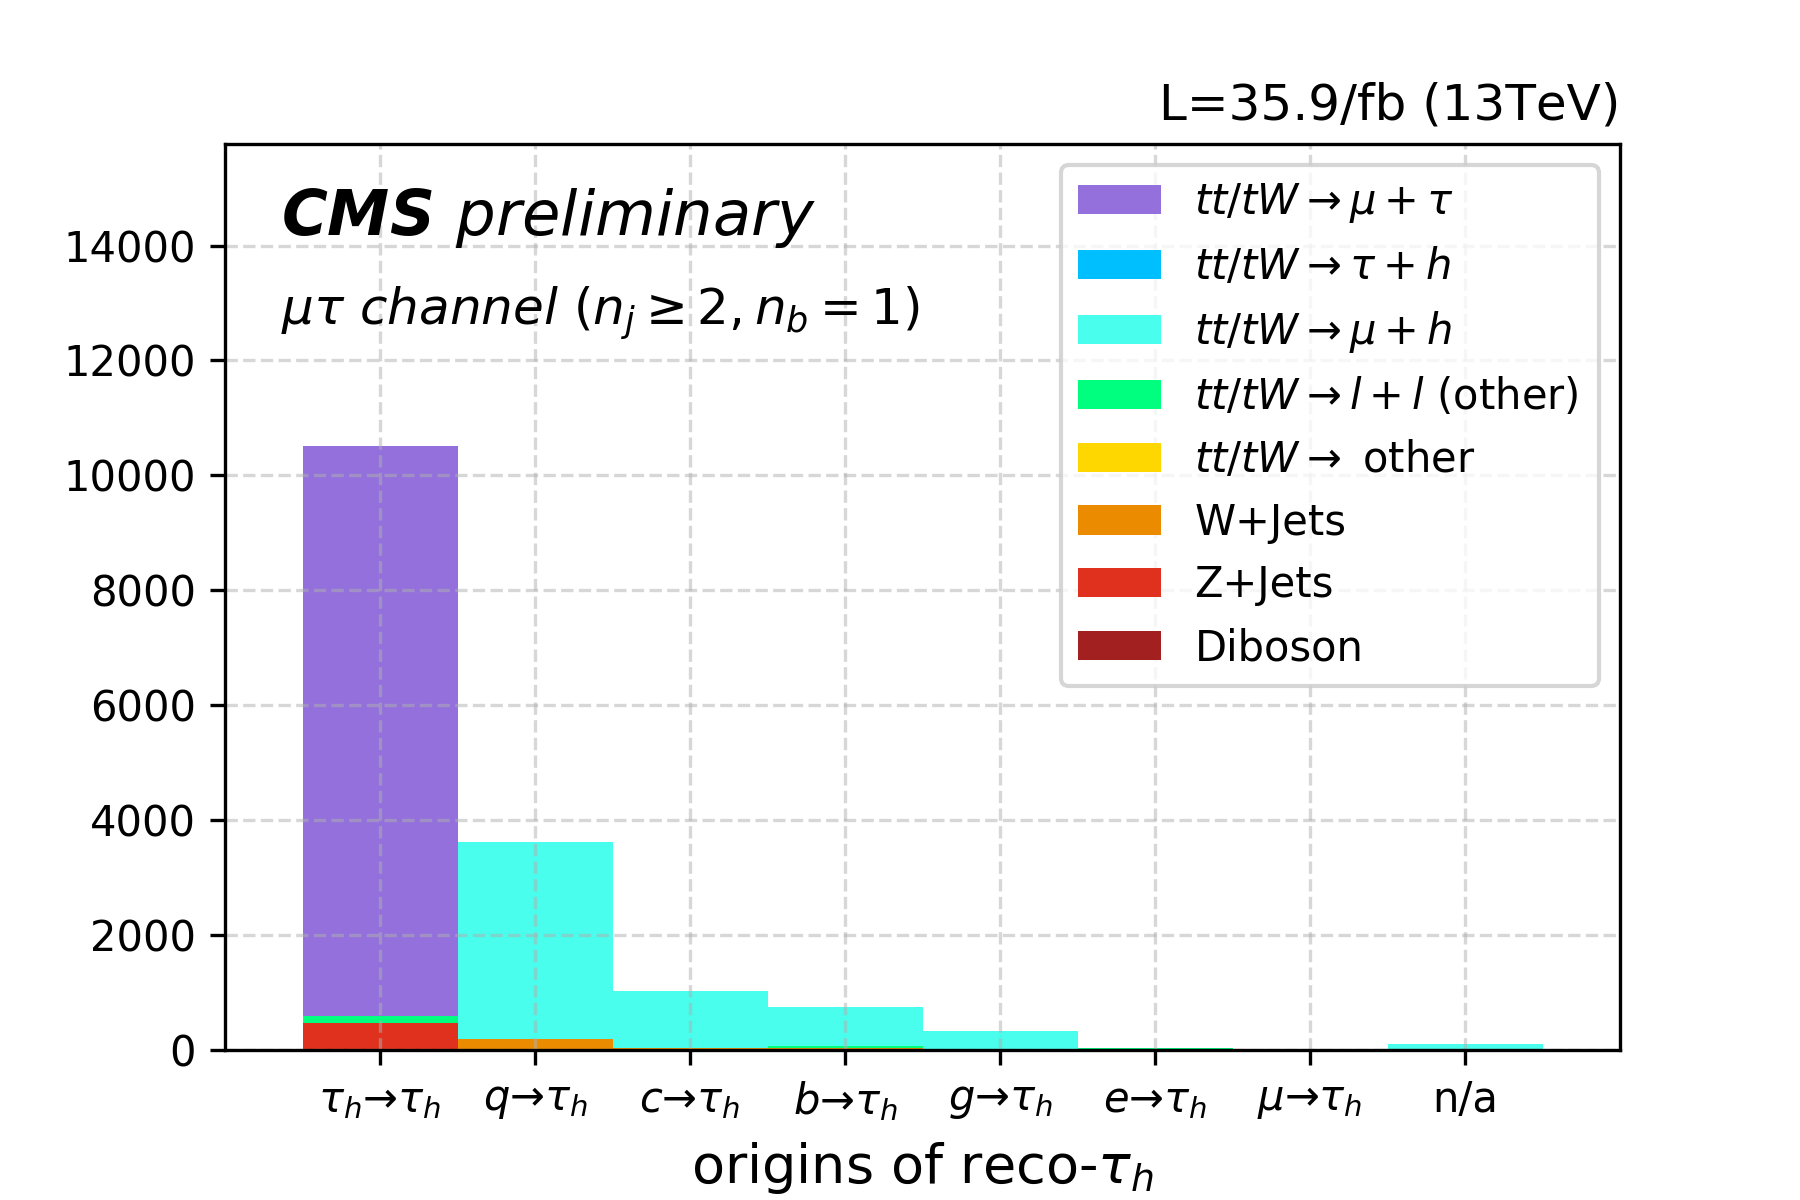
\includegraphics[width=\textwidth]{slides/figures/origin_mutau_1b.png}
        \end{block}
        
        \column{0.55\textwidth}
        \begin{itemize}
            \item Perform a customized measurement of scale factors accounting for the difference of the $j\to \PGth$ fake rate in data and simulation.
            \item $SF_{j \to \PGth}(\pt)$ is measured in $j \to \PGth$ enriched regions:
            \begin{itemize}
            \smaller
                \item \alert{$\cee/\cmm + \PGth$} dominated by \zjets, enriched with light jet faking \PGth;
                \item \alert{$\cem + \PGth$} dominated by \ttbar, enriched with b jet faking \PGth.
            \end{itemize}
            \item The origins of \PGth are found by matching with gen-level particles.
            \item Both Tight and VTight \PGth identification working points are considered.
            \item Systematic uncertainties include luminosity, cross-sections, \Pe/\PGm selection efficiencies.
        \end{itemize}
        \begin{center}
           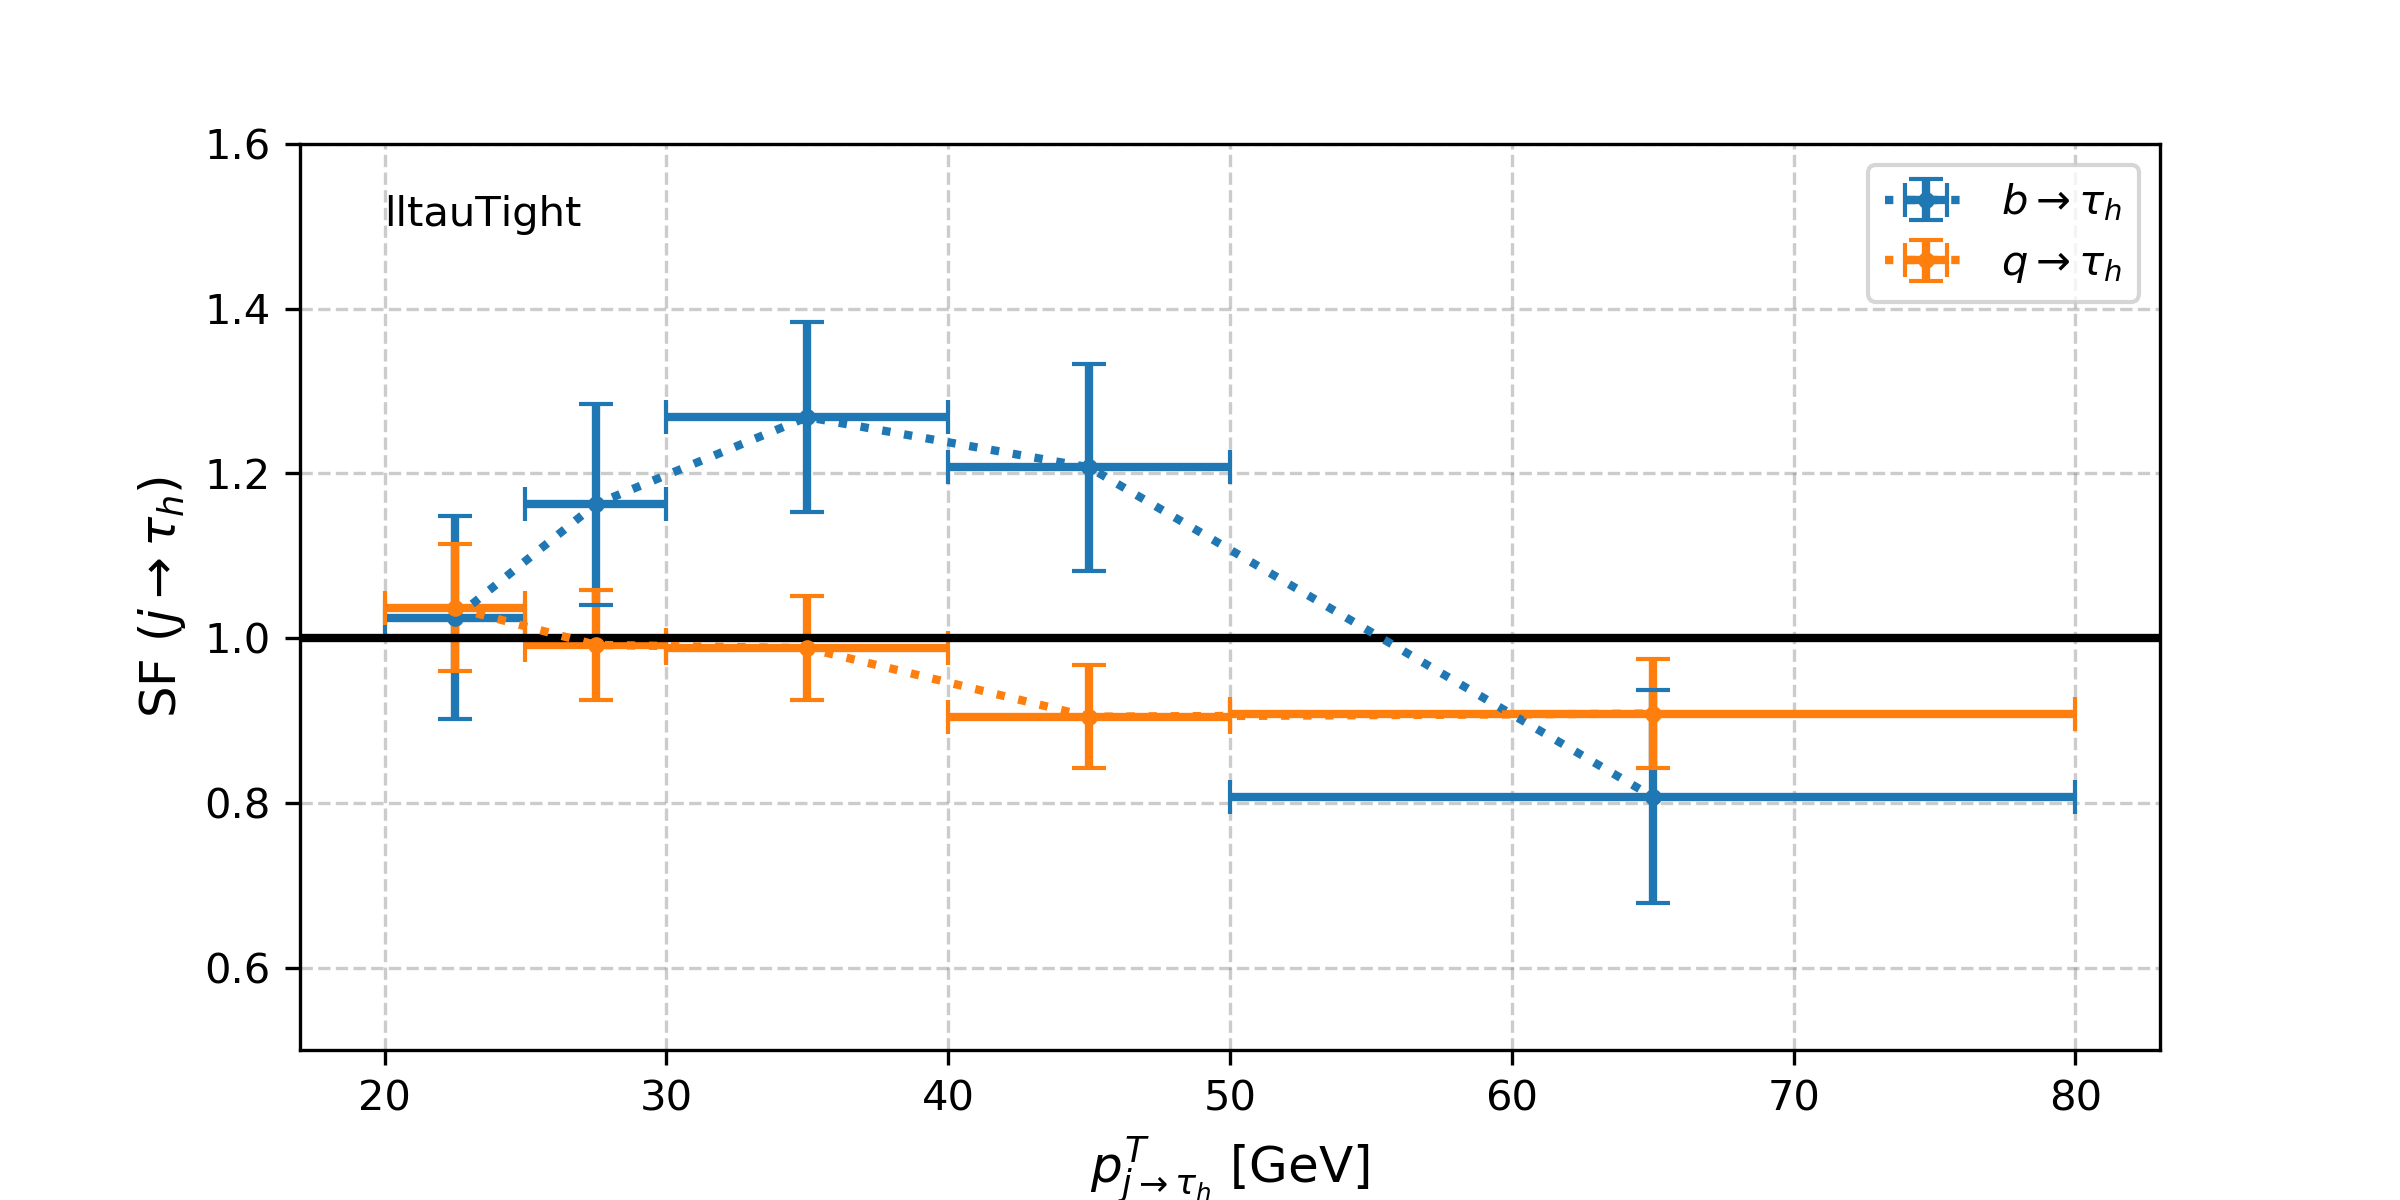
\includegraphics[width=0.8\textwidth]{chapters/Analysis/sectionCalibration/figures/jetToTauh/fit2_ptflavor2_lltauTight.png} 
        \end{center}
        
        
    \end{columns}
    
\end{frame}



\subsection{QCD Estimation}

\begin{frame}{QCD estimation}
\smaller \smaller
    \begin{block}{\cmt and \cet}
    \begin{columns}[c]
        \column{0.7\textwidth}
        \begin{itemize}
            \item Estimated by $n_{\rm data} - \sum n_{\rm MC}$ in the side-band region with \textcolor{red}{same-sign} leptons.
            \item Scale the estimation with a transfer factor \textcolor{blue}{$SF^{\rm SS \to OS}$} measured separately in orthogonal regions: 
            \begin{itemize} 
            \smaller
                \item counting: $\ell \PGth$ with $n_j\geq2,n_b=0$;
                \item shape: $\ell \PGth$ with anti-iso $\ell$ and $n_j=0,n_b=0$.
            \end{itemize}
            % \item Assign 25\% uncertainty to the normalization. [double c]
        \end{itemize}
        
        \column{0.3\textwidth}
        \centering
        \cmt $n_j=0,n_b=0$
        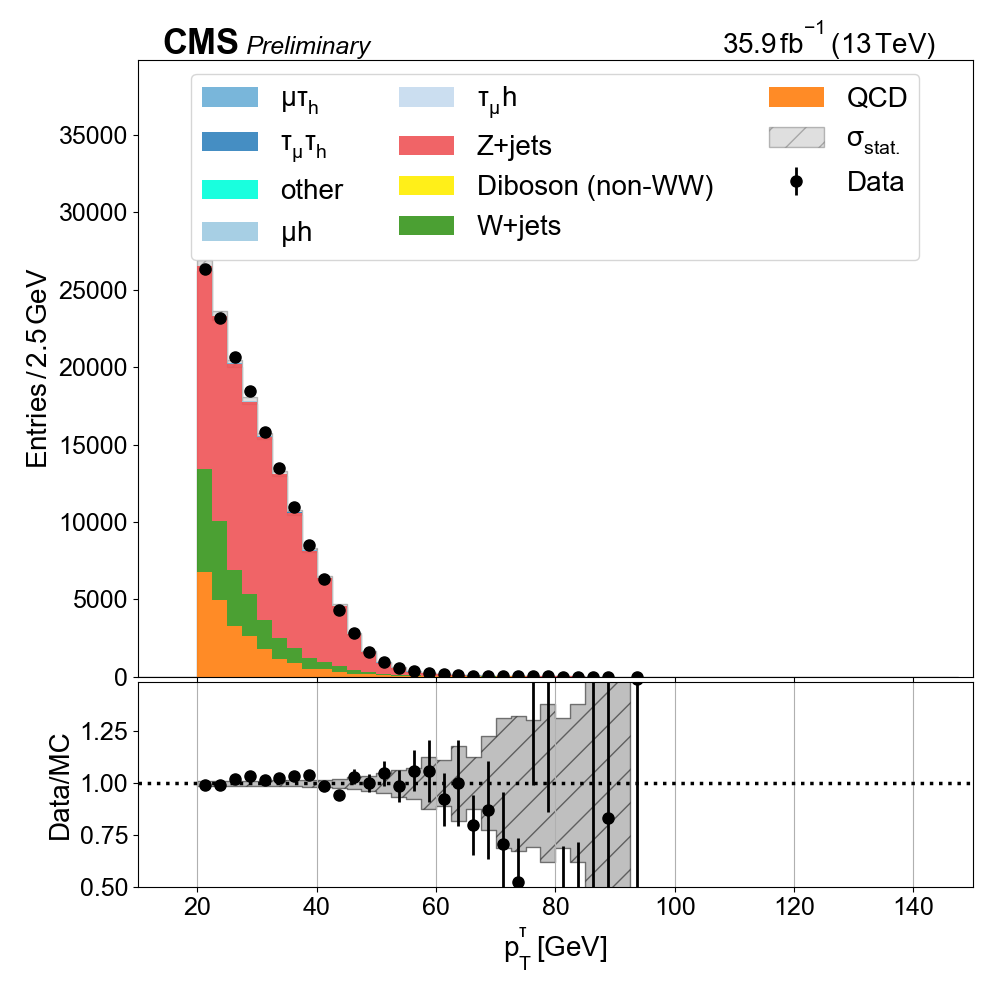
\includegraphics[width=0.8\textwidth]{chapters/Analysis/sectionPlots/figures/data_mc_overlays/mutau_2016_cat_eq0_eq0_signal_linear_lepton_lepton2_pt.png}
    \end{columns}
    \end{block}
    
    

    \begin{block}{\cmh and \ceh}
    \begin{columns}[c]
        \column{0.7\textwidth}
    
        \begin{itemize}
            \item Estimated by $n_{\rm data} - \sum n_{\rm MC}$ in the side-band region with \textcolor{red}{anti-isolated} leptons.
            \item Anti-isolated leptons requires passing Loose but not Tight isolation working point.
            \item Scale the estimation with a transfer factor \textcolor{blue}{ $SF^{\rm \overline{iso} \to iso} (\pt, \eta)$}, measured separately in orthogonal regions ($\ell h$ with $1\leq n_j \leq3, n_b=1$).
            % \item ??? estimation in \ceh is re-normalized by HT-binned QCD ???
            % \item Assign 25\% uncertainty to the normalization. 
        \end{itemize}
        
        \column{0.3\textwidth}
        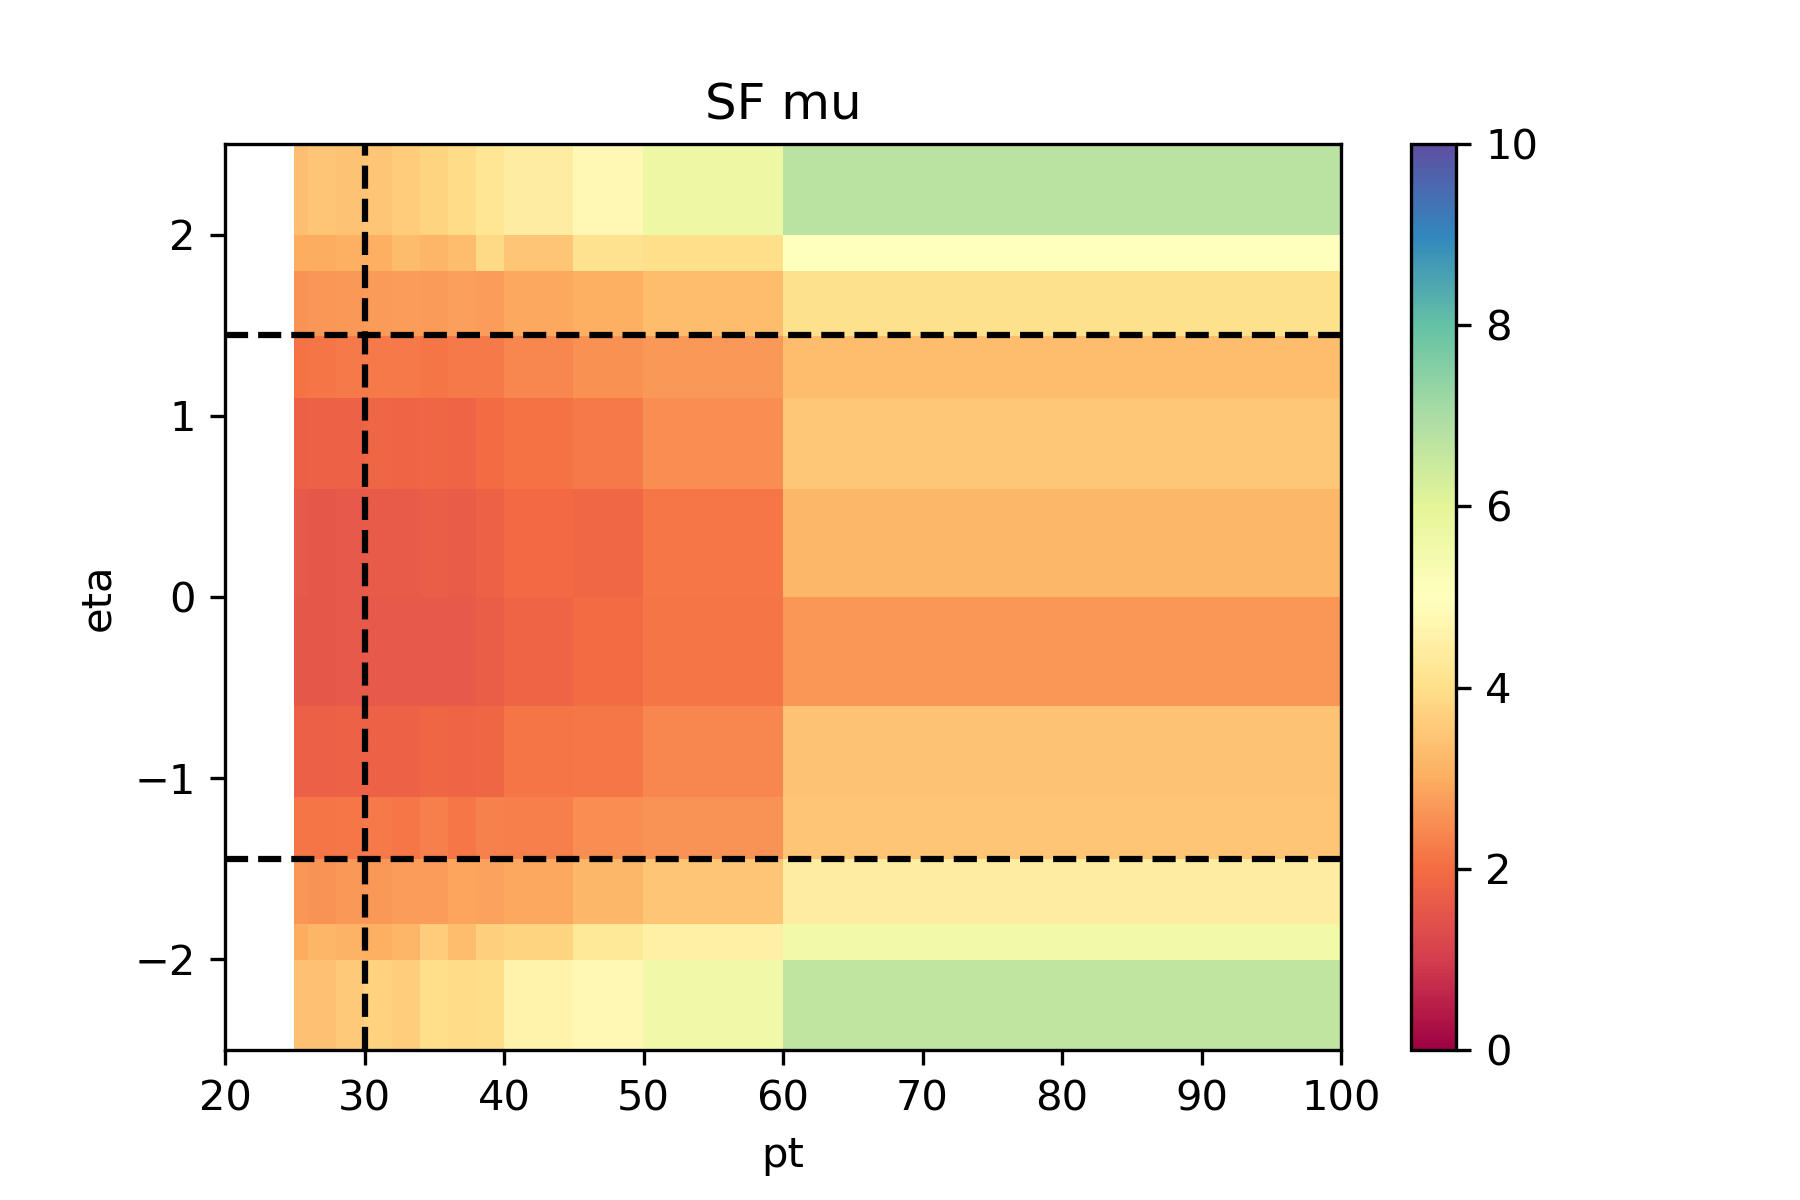
\includegraphics[width=0.95\textwidth,trim=0 0 2cm 0, clip]{chapters/Analysis/sectionBackground/figures/ljets_kinematics/123j1b/SF_mu_2d.png}
        
    \end{columns}
    \end{block}
    
\end{frame}

    
    

    % \begin{center}
    %     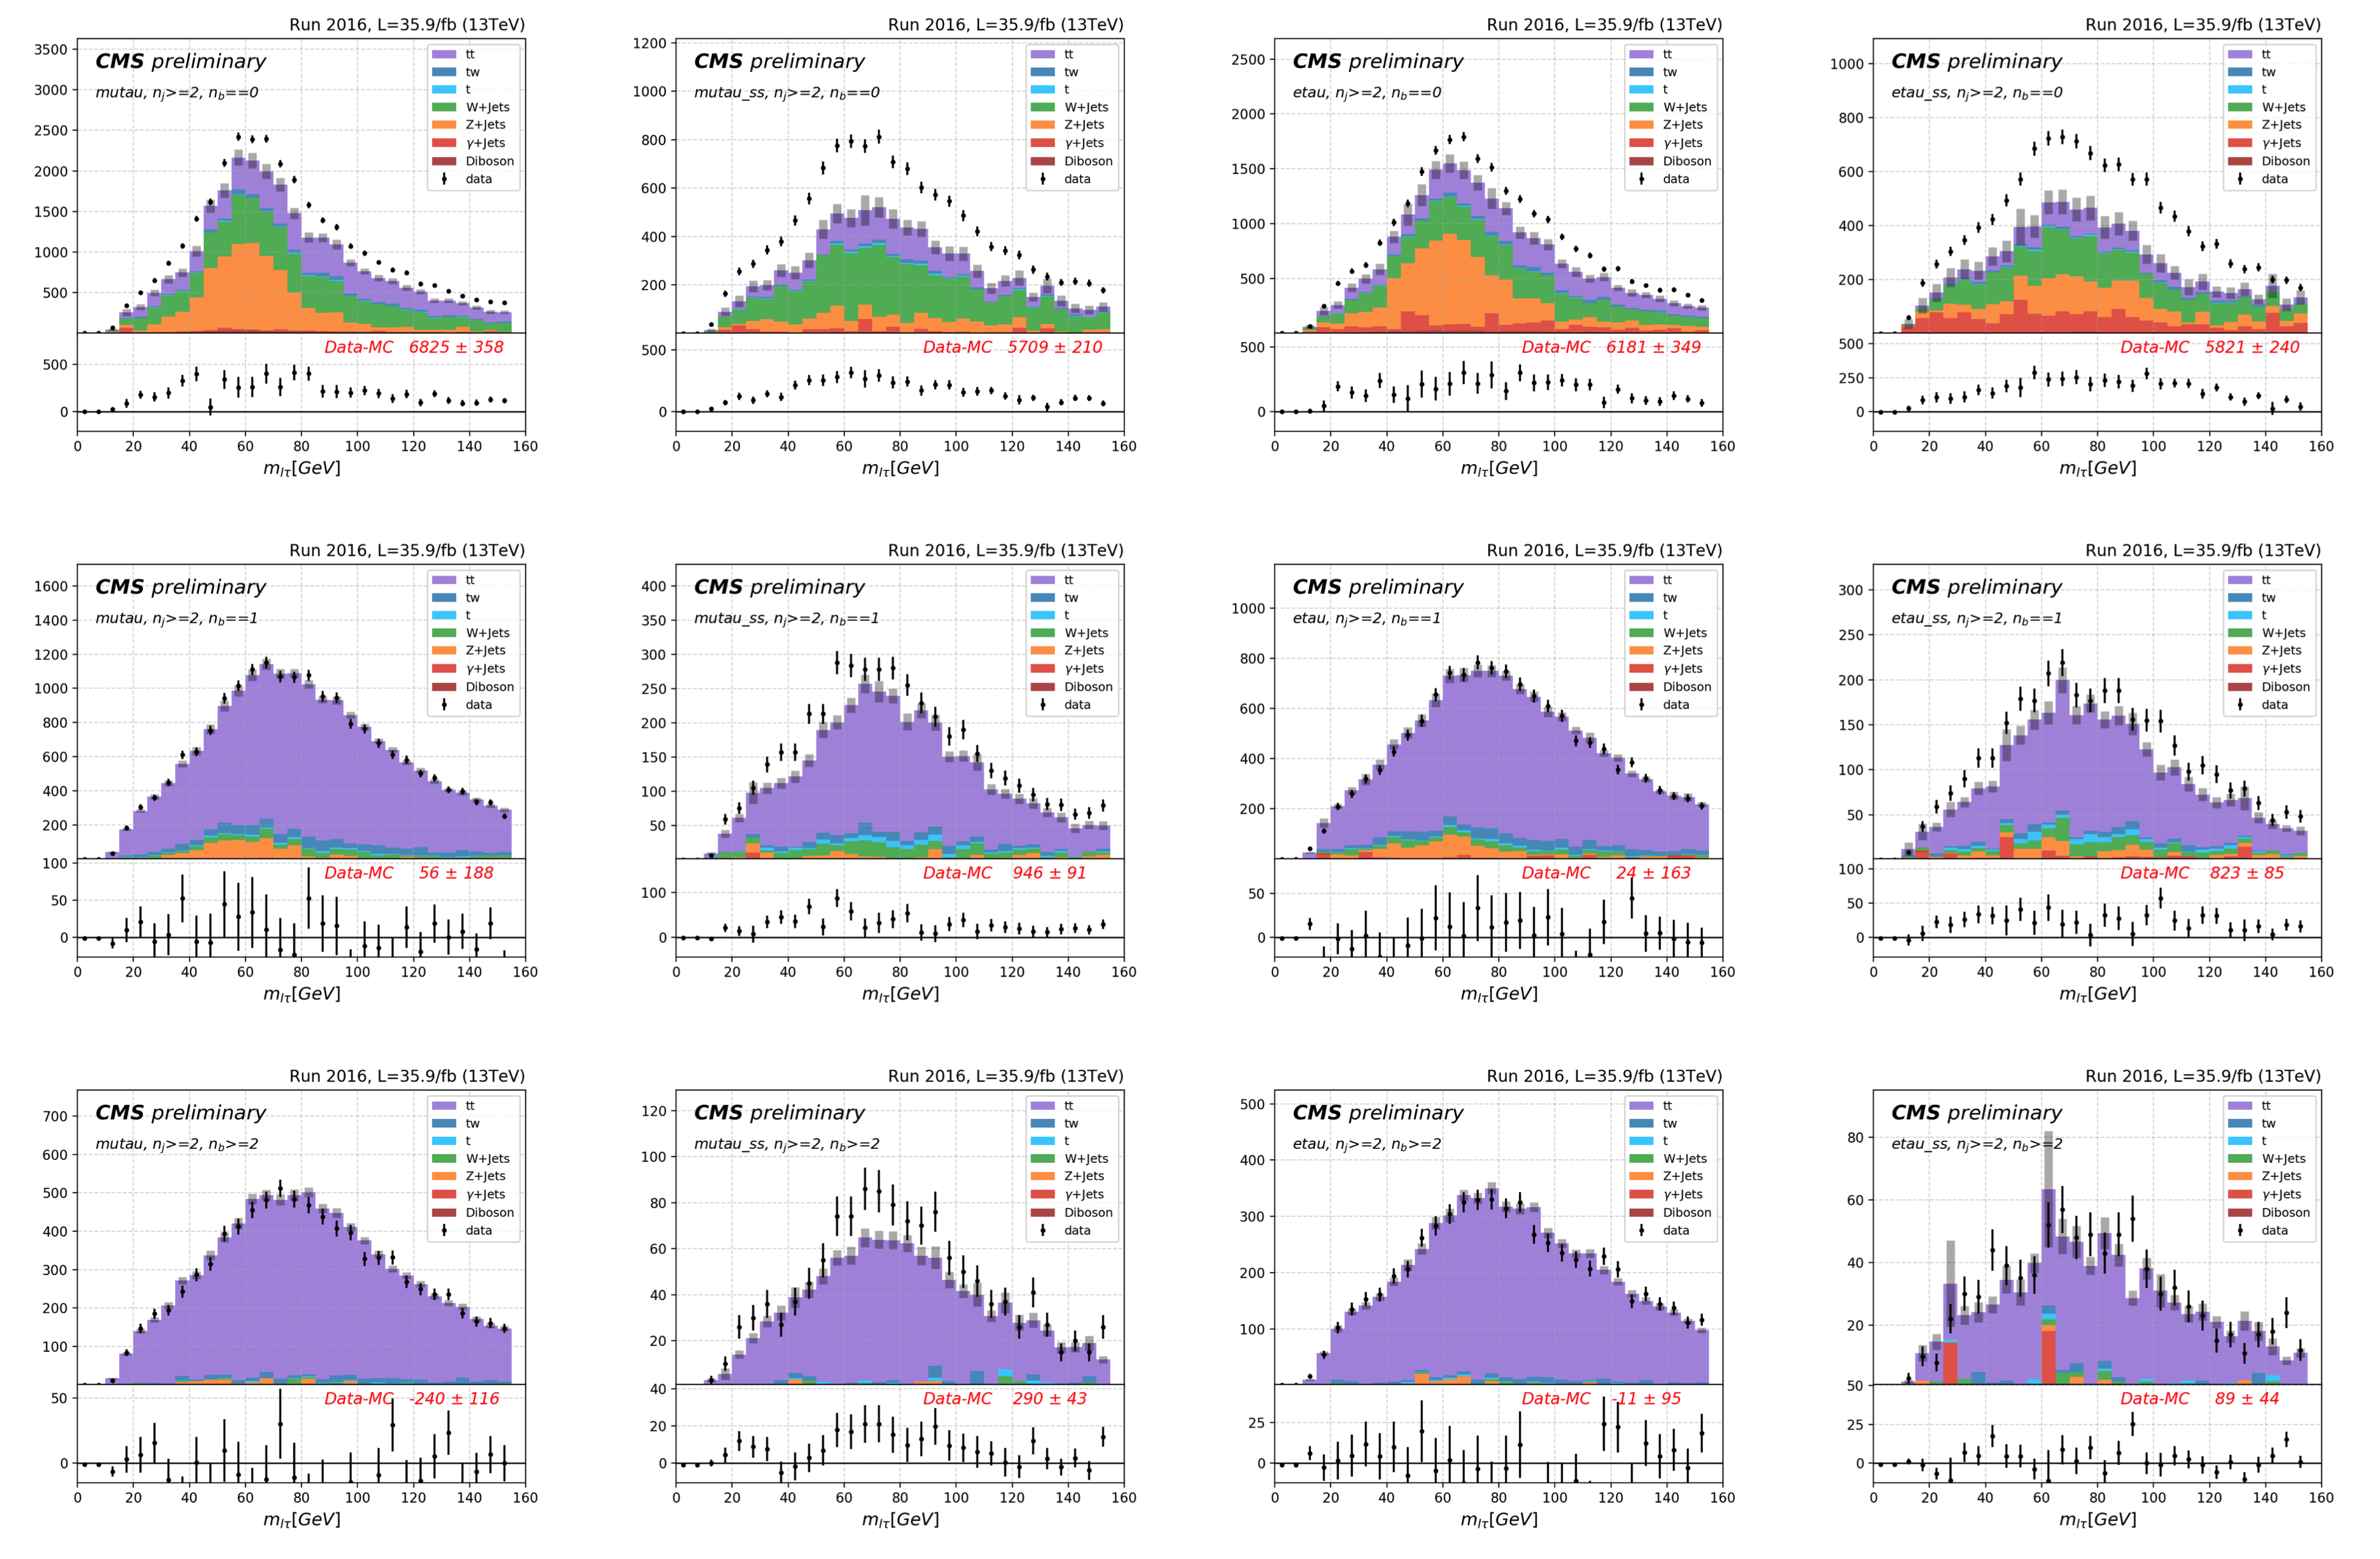
\includegraphics[width=0.9\textwidth, trim=0 21cm 32cm 18cm, clip]{chapters/Analysis/sectionBackground/figures/ltau_kinematics/ltau2.png}
    % \end{center}
    
    % normalization from 2j0b and iso-0j0b








